%@TheDoctorRAB
%
%presentation template for class slides and research presentations
%allows for citations in slide and a list at the end
%
%%%%%
%
%REFERENCES
%
%neup.bst - numbered citations in order of appearance, short author list with et al in reference section
%nsf.bst - numbered citations in order of appearance, full author list in references section
%standard.bst - citations with author last name with et al for more than 2 authors; full author list in references section
%ans.bst is for ANS only. 
%
%author = {Lastname, Firstname and Lastname, Firstname and Lastname, Firstname} for all bst formats
%bst renders the author list itself
%
%author = {{Nuclear Regulatory Commission}} if the author is an organization, institution, etc., and not people
%
%title = {{}} for all
%
%for all - use \citep{-} - [1] or (Borrelli, 2021) in the text
%standard.bst \cite{-} - Borrelli (2021) in the text
%standard.bst lists references alphabetically
%the rest list numerically
%
%
%%% citations on slides 
%
%\citep{xxxnna} where the citation should go
%\blfootnote{\fontsize\cite{xxxnna}\fontsize\bibentry{xxxnna}} before \end{frame}
%
%
%%%%%

%%%%% presentation settings
\documentclass[aspectratio=1610,pdftex,dvipsnames,compress,xcolor={dvipsnames}]{beamer}
\usetheme{Boadilla}
\usecolortheme{seahorse}
\beamertemplatenavigationsymbolsempty
\addtobeamertemplate{footnote}{\hskip -2em}{} %pushes footnote to margin
%%% font style - can add size, etc.
%https://tug.ctan.org/macros/latex/contrib/beamer/doc/beameruserguide.pdf
\setbeamerfont{title}{series=\bfseries}
\setbeamerfont{frametitle}{series=\bfseries}
\setbeamerfont{footline}{series=\bfseries}
\setbeamerfont{author}{series=\bfseries}
\setbeamerfont{institute}{series=\bfseries}
\setbeamerfont{date}{series=\bfseries}
\setbeamertemplate{page number in head/foot}[framenumber] %just gives slide number; comment out for 1/7, 2/7...
%%%%%


%%%%% colors
%http://latexcolor.com/
%https://en.wikibooks.org/wiki/LaTeX/Colors#:~:text=black%2C%20blue%2C%20brown%2C%20cyan,be%20available%20on%20all%20systems.
%sam root
\definecolor{BackGround}{RGB}{255,250,240}
\definecolor{PrideGold}{RGB}{241,179,0}
\definecolor{Silver}{RGB}{165,169,180}
\definecolor{White}{RGB}{255,255,255}
\definecolor{Black}{RGB}{25,25,25}
\definecolor{Chrome}{RGB}{245,245,245}
%%% general
\definecolor{aliceblue}{rgb}{0.94, 0.97, 1.0}
\definecolor{antiquewhite}{rgb}{0.98, 0.92, 0.84}
\definecolor{lightmauve}{rgb}{0.86, 0.82, 1.0}
\definecolor{brilliantlavender}{rgb}{0.96, 0.73, 1.0}
\definecolor{brandeisblue}{rgb}{0.0, 0.44, 1.0}
\definecolor{darkmidnightblue}{rgb}{0.0, 0.2, 0.4}
\definecolor{darkchampagne}{rgb}{0.76, 0.7, 0.5}
%%% set slides
\setbeamercolor{background canvas}{bg=BackGround}
%%%
\setbeamercolor{block title}{bg=Silver,fg=Black}
\setbeamercolor{block body}{bg=Silver!20,fg=Black}
\setbeamercolor{block title alerted}{bg=Black,fg=Silver}
\setbeamercolor{block body alerted}{bg=PrideGold,fg=Black}
\setbeamercolor{alerted text}{fg=Silver}
\setbeamercolor*{block title example}{bg=PrideGold,fg=Black}
\setbeamercolor*{block body example}{bg=PrideGold!20,fg=Black}
%%%
\setbeamercolor*{palette primary}{bg=PrideGold,fg=Black}
\setbeamercolor*{palette secondary}{bg=PrideGold,fg=Black}
\setbeamercolor*{palette tertiary}{bg=PrideGold,fg=Black}
%%%
\setbeamercolor*{titlelike}{bg=PrideGold,fg=Black}
\setbeamercolor*{title}{bg=PrideGold,fg=Black}
\setbeamercolor*{item}{fg=PrideGold}
\setbeamercolor*{caption name}{fg=PrideGold}
%%%
\setbeamercolor*{sidebar}{fg=PrideGold,bg=Black}
\setbeamercolor*{title in sidebar}{fg=PrideGold}
\setbeamercolor*{author in sidebar}{fg=PrideGold}
\setbeamercolor*{section in sidebar}{fg=PrideGold}
%%%
\setbeamercolor{section in toc}{fg=Black}
\setbeamercolor{subsection in toc}{fg=Black}
%%%
\setbeamercolor{page number in head/foot}{fg=Black,bg=PrideGold}
%\setbeamercolor{footline}{bg=Black}
%%%
\setbeamercolor{bibliography entry author}{fg=Black}
\setbeamercolor{bibliography entry note}{fg=Black}
\setbeamercolor{bibliography entry title}{fg=Black}
%%%
\newcommand{\x}{\cellcolor{aliceblue}} %use to shade in table cell
\newcommand{\y}{\cellcolor{lightgray}} %use to shade in table cell
\newcommand{\z}{\cellcolor{antiquewhite}} %use to shade in table cell
\newcommand{\w}{\cellcolor{darkchampagne}} %use to shade in table cell

%%%%%


%%%%% general 
%\documentclass[11pt,a4paper]{article}
%\usepackage[lmargin=1in,rmargin=1in,tmargin=1in,bmargin=1in]{geometry}
\usepackage[pagewise]{lineno} %line numbering
\usepackage{setspace}
\usepackage{ulem} %strikethrough - do not \sout{\cite{}}
\usepackage{graphicx}
\usepackage{mypythonhighlight,verbatim}
\usepackage{filecontents}
\usepackage{tablefootnote}
\usepackage{footnotehyper}
\usepackage{float}
%\usepackage{subfig}
\usepackage[yyyymmdd]{datetime} %date format
\renewcommand{\dateseparator}{.}
\graphicspath{{$TEXIMG/}} %path to graphics
\setcounter{secnumdepth}{5} %set subsection to nth level
\usepackage{needspace}
\usepackage[stable,hang,flushmargin]{footmisc} %footnotes in section titles and no indent; standard.bst
\usepackage[inline]{enumitem}
\setlist[itemize]{label=\textbullet}
\usepackage{boldline}
\usepackage{makecell}
\usepackage{booktabs}
\usepackage{amssymb}
\usepackage{gensymb}
\usepackage{amsmath,nicefrac}
\usepackage{physics}
\usepackage{lscape}
\usepackage{array}
\usepackage{chngcntr}
\usepackage{hyperref}
\hypersetup{colorlinks,linkcolor=black,citecolor=black,urlcolor=blue} 
%\usepackage{sectsty}
\usepackage{textcomp}
\usepackage{lastpage}
\usepackage{xargs} %for \newcommandx
\usepackage[colorinlistoftodos,prependcaption,textsize=tiny]{todonotes} %makes colored boxes for commenting
\usepackage{soul}
\usepackage{color}
\usepackage{marginnote}
\usepackage[figure,table]{totalcount}
\usepackage[capitalise]{cleveref}
\usepackage{microtype} %improves typography for pdf
\usepackage[pdftex,dvipsnames]{colortbl} %change font color
%%%%%


%%%%% tikz
\usepackage{pgf}
\usepackage{tikz} % required for drawing custom shapes
\usetikzlibrary{shapes,arrows,automata,trees}
%%%%%


%%%%% fonts
\usepackage{times}
%\renewcommand{\sfdefault}{ubuntu}
%arial - uncomment next two lines
%\usepackage{helvet}
%\renewcommand{\familydefault}{\sfdefault}
%%%%%


%%%%% references
%\usepackage[round,semicolon]{natbib} %for (Borrelli 2021; Clooney 2019) - standard.bst 
\usepackage[numbers,sort&compress]{natbib} %for [1-3] - nsf.bst, neup.bst
\usepackage{bibentry}
\setlength{\bibsep}{7pt} %sets space between references
%\renewcommand{\bibsection}{} %suppresses large 'references' heading
%\renewcommand\bibpreamble{\vspace{\baselineskip}} %sets spacing after heading if not using default references heading
%%%%%


%%%%% tables and figures
\usepackage{longtable} %need to put label at top under caption then \\ - use spacing
\usepackage{makecell}
\usepackage{tablefootnote}
\usepackage{tabularx}
\usepackage{multirow}
\usepackage{tabto} %general tabbed spacing
\usepackage{pdfpages}
\usepackage{wrapfig} %wraps figures around text
\setlength{\intextsep}{0.00mm}
\setlength{\columnsep}{1.00mm}
\usepackage[singlelinecheck=false,labelfont=bf]{caption}
\usepackage{subcaption}
\captionsetup[table]{justification=justified,skip=5pt,labelformat={default},labelsep=period,name={Table}} %sets a space after table caption
\captionsetup[figure]{justification=justified,skip=5pt,labelformat={default},labelsep=period,name={Figure}} %sets space above caption, 'figure' format
\captionsetup[wrapfigure]{justification=centering,aboveskip=0pt,belowskip=0pt,labelformat={default},labelsep=period,name={Fig.}} %sets space above caption, 'figure' format
\captionsetup[wraptable]{justification=centering,aboveskip=0pt,belowskip=0pt,labelformat={default},labelsep=period,name={Table}} %sets space above caption, 'figure' format
%%%%%


%%%%% watermark
%\usepackage[firstpage,vpos=0.63\paperheight]{draftwatermark}
%\SetWatermarkText{\shortstack{DRAFT\\do not distribute}}
%\SetWatermarkScale{0.20}
%%%%%


%%%%% cross referencing files
%\usepackage{xr} %for revisions - will cross reference from one file to here
%\externaldocument{/path/to/auxfilename} %aux file needed
%%%%%


%%%%% toc and glossaries
\usepackage[toc,title]{appendix}
\usepackage[acronym,nomain,nonumberlist]{glossaries}
%\makenoidxglossaries
%\usepackage{titlesec,titletoc}
%\renewcommand{\thepart}{ARTICLE \Roman{part}} %puts the label into the command so \thelabel will carry through
%\renewcommand{\thesection}{\arabic{section}} %puts the label into the command so \thelabel will carry through
%\titleformat{\part}{\normalfont\large\bfseries}{\thepart}{}{}[]
%\titlespacing*\part{0pt}{0.95\baselineskip}{0.75\baselineskip}
%\titleformat{\section}[runin]{\normalfont\large\bfseries}{\thesection}{-1em}{}[.]
%\titlespacing*\section{0pt}{0.65\baselineskip}{0.55\baselineskip}
%\titleformat{\subsection}[runin]{\normalfont\normalsize\bfseries}{\thesubsection}{-1em}{}[.]
%\titlespacing*\subsection{0pt}{0.50\baselineskip}{0.35\baselineskip}
%\titleformat{\paragraph}[runin]{\normalfont\normalsize\bfseries\itshape}{\theparagraph}{-1em}{}[.]
%\titlespacing*\paragraph{0pt}{0.45\baselineskip}{0.25\baselineskip}
%\titleformat{\subparagraph}[runin]{\normalfont\normalsize\itshape}{\thesubparagraph}{-1em}{}[.]
%\titlespacing*\subparagraph{0pt}{0.40\baselineskip}{0.25\baselineskip}
%\titleformat{\paragraph}[hang]{\normalfont\normalsize\bfseries}{\theparagraph}{5pt}{}[]
%\titlespacing*\paragraph{0pt}{0.50\baselineskip}{0.25\baselineskip}
%\titleformat{\subparagraph}[runin]{\normalfont\normalsize\itshape}{\thesubparagraph}{-1em}{}[.]
%\titlespacing*\subparagraph{0pt}{0.40\baselineskip}{0.20\baselineskip}
%%%%%


%%%%% editing
\newcommand{\edit}[1]{\textcolor{blue}{#1}} %shortcut for changing font color on revised text
\newcommand{\fn}[1]{\footnote{#1}} %shortcut for footnote tag
\newcommand*\sq{\mathbin{\vcenter{\hbox{\rule{.3ex}{.3ex}}}}} %makes a small square as a separator $\sq$
%\newcommand{\sk}[1]{\sout{#1}} %shortcut for default strikethrough - do not sk through citep
\newcommand\sk{\bgroup\markoverwith{\textcolor{red}{\rule[0.5ex]{1pt}{1pt}}}\ULon} %strikethrough with red line; not in \section{}
%\st{} does strikethrough using soul package but does not like acronyms
\newcommand{\blucell}{\cellcolor{aliceblue}} %use to shade in table cell
\newcommand{\grycekk}{\cellcolor{lightgray}} %use to shade in table cell
\newcommand{\whicell}{\cellcolor{antiquewhite}} %use to shade in table cell
%%%%%


%%%%% acronyms
\newcommand{\acf}{\acrfull} %full acronym
\newcommand{\acl}{\acrlong} %long acronym
\newcommand{\acs}{\acrshort} %short acronym

\newcommand{\acfp}{\acrfullpl} %full acronym plural
\newcommand{\aclp}{\acrlongpl} %long acronym plural
\newcommand{\acsp}{\acrshortpl} %short acronym plural
%%%%%


%%%%% todonotes
\newcommandx{\cmt}[2][1=]{\todo[author=\textbf{STRUCTURE},tickmarkheight=0.15cm,linecolor=red,backgroundcolor=red!25,bordercolor=black,#1]{#2}}
\newcommandx{\con}[2][1=]{\todo[author=\textbf{CONTENT},tickmarkheight=0.15cm,linecolor=brilliantlavender,backgroundcolor=brilliantlavender,bordercolor=black,#1]{#2}}
%\newcommandx{\rab}[2][1=]{\todo[noline,author=\textbf{RAB},backgroundcolor=Plum!25,bordercolor=black,#1]{#2}}
%%%
%\newcommandx{\jon}[2][1=]{\todo[noline,author=\textbf{ATTN: Johnson},backgroundcolor=blue!25,bordercolor=black,#1]{#2}}
%\newcommandx{\han}[2][1=]{\todo[noline,author=\textbf{ATTN: Haney},backgroundcolor=OliveGreen!25,bordercolor=black,#1]{#2}}
\newcommandx{\rab}[2][1=]{\todo[author=\textbf{Borrelli},tickmarkheight=0.15cm,linecolor=black,backgroundcolor=Plum!25,bordercolor=black,#1]{#2}}
%\newcommandx{\han}[2][1=]{\todo[author=\textbf{ATTN: Haney},tickmarkheight=0.15cm,linecolor=OliveGreen,backgroundcolor=OliveGreen!25,bordercolor=OliveGreen,#1]{#2}}
%\newcommandx{\jon}[2][1=]{\todo[author=\textbf{ATTN: Johnson},tickmarkheight=0.15cm,linecolor=blue,backgroundcolor=blue!25,bordercolor=blue,#1]{#2}}
%%% highlighting 
\DeclareRobustCommand{\hlc}[1]{{\sethlcolor{LimeGreen}\hl{#1}}}
\makeatletter
    \if@todonotes@disabled
    \newcommand{\hlh}[2]{#1}
    \else
    \newcommand{\hlh}[2]{\han{#2}\hlc{#1}}
    \fi
    \makeatother

\DeclareRobustCommand{\hld}[1]{{\sethlcolor{CornflowerBlue}\hl{#1}}}
\makeatletter
    \if@todonotes@disabled
    \newcommand{\hlj}[2]{#1}
    \else
    \newcommand{\hlj}[2]{\jon{#2}\hld{#1}}
    \fi
    \makeatother

\DeclareRobustCommand{\hlf}[1]{{\sethlcolor{lightmauve}\hl{#1}}}
\makeatletter
    \if@todonotes@disabled
    \newcommand{\hlb}[2]{#1}
    \else
    \newcommand{\hlb}[2]{\rab{#2}\hlf{#1}}
    \fi
    \makeatother
%%%%%


%%%%% table alignments
\newcolumntype{L}[1]{>{\raggedright\let\newline\\\arraybackslash\hspace{0pt}}m{#1}} %uses \raggedright with m,p{} in table column
\newcolumntype{C}[1]{>{\centering\let\newline\\\arraybackslash\hspace{0pt}}m{#1}} %uses \raggedright with m,p{} in table column
\newcolumntype{R}[1]{>{\raggedleft\let\newline\\\arraybackslash\hspace{0pt}}m{#1}} %uses \raggedright with m,p{} in table column
%%%%%


%%%%% table contents
\makeatletter
\renewcommand\tableofcontents{%
    \@starttoc{toc}%
}
\makeatother

\makeatletter
\renewcommand\listoffigures{%
    \@starttoc{lof}%
}
\makeatother

\makeatletter
\renewcommand\listoftables{%
    \@starttoc{lot}%
}
\makeatother

\makeatletter
\newcommand*\ftp{\fontsize{16.5}{17.5}\selectfont}
\makeatother
%%%%%


%%%%% user commands
\newcommand\blfootnote[1]{%
  \begingroup
  \renewcommand\thefootnote{}\footnote{#1}%
  \addtocounter{footnote}{-1}%
  \endgroup
}


\makeatletter
\renewcommand{\@biblabel}[1]{#1.\hfill} %bibliography ordered list has numbers left flush
\makeatother


\AtBeginSection[]{
    \begin{frame}[plain]{}
         
         \vfill

         \centering
         \begin{beamercolorbox}[sep=8pt,center,shadow=true,rounded=true]{titlelike}
             \usebeamerfont{title}\insertsectionhead\par
         \end{beamercolorbox}

         \vfill

     \end{frame}
 }
%%%%%


%%%%% header and footer
%\usepackage{fancyhdr}
%\pagestyle{fancy}
%\fancyhf{} %move page number to bottom right
%\renewcommand{\headrulewidth}{0pt} %set line thickness in header; uncomment as is to remove line
%\lhead{\scriptsize Name}
%\lhead{\scriptsize PNUCENE-D-22-xxxxx}
%\chead{\scriptsize \textit{PhD White Paper Project Proposal}}
%\rhead{\scriptsize \today}
%\rfoot{\thepage}
%%%%%


%%%%% acronyms
\input{$ACRONYM/acronyms}
%%%%%

%%%%% spacing
%\onehalfspacing %linespacing
%\setstretch{1.05} %linespacing
%\spacing{1.25} %equivalent to 1.5 line spacing in Word
%%%%%


%%%%% linenumbering
%\linenumbers %toggle line numbers
%\pagewiselinenumbers %reset line numbers on new page
%\modulolinenumbers[1] %line numbering interval
%%%%%


%%%%% title page
\addtocounter{framenumber}{-1} %does not count the title slide in the slide count
\title[NE585 - Nuclear fuel cycles]{NE585\\NUCLEAR FUEL CYCLES\\Nuclear reactor theory\\4}
\author[@TheDoctorRAB]{R. A. Borrelli}
\institute[]{
    \acl{ui}\\
    \vspace{0.10in}
    
\includegraphics[width=0.20\textwidth]{logo/university-of-idaho/nuclear-engineering/ne-logo.png}
    }
\date{\acl{iff}}
%%%%%


\begin{document}


%%%%% title page with no footer
{
    \setbeamertemplate{footline}{}
    \begin{frame}
        \titlepage
    \end{frame}
}
%%%%%


\begin{frame}{Learning objectives}
    \begin{enumerate}[series=outerlist,topsep=0pt,itemsep=21pt,leftmargin=*,label=(\arabic*)]
        \item[]Design a critical nuclear reactor configuration
        \item[]Derive steady state neutron transport equation
        \item[]Demonstrate transient reactor behavior
        \item[]\href{https://uidaho.pressbooks.pub/nuclearengineering/chapter/front-end-of-the-fuel-cycle-2/}{Watch videos on different reactors and historical events}
    \end{enumerate}
\end{frame}


\begin{frame}{Learning nodes}
    \begin{columns}[t]

        \begin{column}{0.50\textwidth}
            \begin{enumerate}[series=outerlist,topsep=0pt,itemsep=1pt,leftmargin=*,label=(\arabic*)]
                \item[]\textbf{Review}
                    \vspace{0.10in}
                \item[]\textbf{Neutron chain reaction}
                    \vspace{0.10in}
                \item[]\textbf{Neutron multiplication factor}
                \item[]Four factor formula
                \item[]Neutron reproduction factor
                \item[]Fuel utilization factor
                \item[]Resonance escape probability
                \item[]Fast fission factor
                    \vspace{0.10in}
                \item[]\textbf{Critical and subcritical configurations}
                    \vspace{0.10in}
                \item[]\textbf{Burnup}
                    \vspace{0.10in}
                \item[]\textbf{Neutron interaction rate}
                    \vspace{0.10in}
                \item[]\textbf{Neutron diffusion}
            \end{enumerate}
        \end{column}

        \begin{column}{0.50\textwidth}
            \begin{enumerate}[series=outerlist,topsep=0pt,itemsep=1pt,leftmargin=*,label=(\arabic*)]
                \item[]\hfill\textbf{Equation of continuity}
                    \vspace{0.10in}
                \item[]\hfill\textbf{Diffusion equation}
                    \vspace{0.10in}
                \item[]\hfill\textbf{Diffusion length}
                    \vspace{0.10in}
                \item[]\hfill\textbf{Group diffusion theory}
            \end{enumerate}
        \end{column}

    \end{columns}
\end{frame}


\begin{frame}{More learning nodes}
    \begin{columns}[t]

        \begin{column}{0.50\textwidth}
            \begin{enumerate}[series=outerlist,topsep=0pt,itemsep=1pt,leftmargin=*,label=(\arabic*)]
                \item[]\textbf{Nuclear reactor design}
                \item[]One group reactor equation
                \item[]Buckling
                \item[]Leakage
                \item[]Criticality for thermal reactors
                \item[]Two group theory
                \item[]Six factor formula
                \item[]Reflected reactor
                \item[]Multigroup theory
                \item[]Heterogeneity
            \end{enumerate}
        \end{column}

        \begin{column}{0.50\textwidth}
            \begin{enumerate}[series=outerlist,topsep=0pt,itemsep=1pt,leftmargin=*,label=(\arabic*)]
                \item[]\hfill\textbf{Reactor kinetics}
                \item[]\hfill Prompt neutrons
                \item[]\hfill Delayed neutrons
                \item[]\hfill Reactor period
                \item[]\hfill Point kinetics equations
                \item[]\hfill Prompt critical
                    \vspace{0.15in}
                \item[]\hfill\textbf{Temperature coefficient}
                    \vspace{0.15in}
                \item[]\hfill\textbf{Doppler broadening}
                    \vspace{0.15in}
                \item[]\hfill\textbf{Void coefficient}
                    \vspace{0.15in}
                \item[]\hfill\textbf{Fission product poisons}
            \end{enumerate}
        \end{column}

    \end{columns}
\end{frame}


\begin{frame}{Even more learning nodes}
    \begin{enumerate}[series=outerlist,topsep=0pt,itemsep=1pt,leftmargin=*,label=(\arabic*)]
                \item[]\textbf{Heat removal}
                \item[]Heat removal rate
                \item[]Heat production rate
                \item[]Conduction
                \item[]Convection
                    \vspace{0.15in}
                \item[]\textbf{Dimensionless heat transfer numbers}
                    \vspace{0.15in}
                \item[]\textbf{Boiling}
                    \vspace{0.15in}
                \item[]\textbf{Meltdown}
    \end{enumerate}
\end{frame}


\section{Nuclear fuel cycle review}


\addtocounter{framenumber}{-1} 
\begin{frame}{}
    \begin{figure}
        \centering
        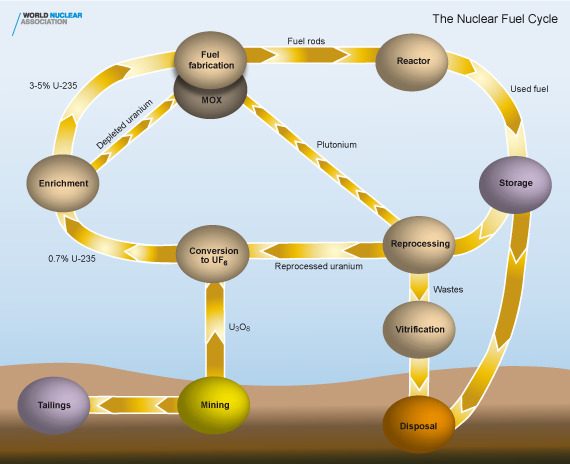
\includegraphics[width=0.75\textwidth]{ne585/nuclear.fuel.cycle1.jpg}
%        \caption{}
    \end{figure}
\end{frame}


\section{Neutron chain reaction}


\addtocounter{framenumber}{-1} 
\begin{frame}{Designing a nuclear reactor is about controlling the neutron chain reaction}
    \begin{figure}
        \centering
        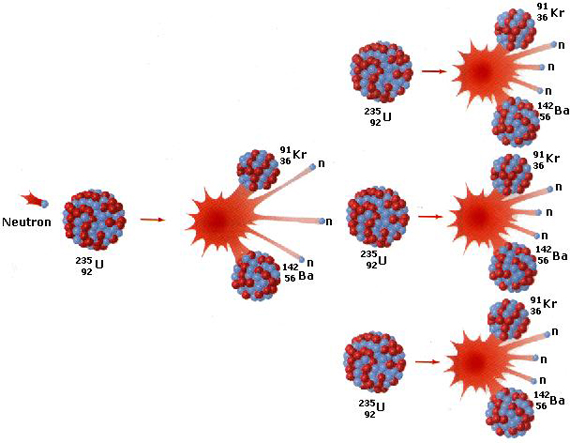
\includegraphics[width=0.75\textwidth]{ne585/fission.jpg}
%        \caption{}
    \end{figure}
\end{frame}


\section{Neutron multiplication factor}


\addtocounter{framenumber}{-1} 
\begin{frame}{The neutron multiplication factor describes a chain reaction}
    \begin{enumerate}[series=outerlist,topsep=0pt,itemsep=21pt,leftmargin=*,label=(\arabic*)]
        \item[]Ratio of fissions in generation $(n+1)$ to fissions in generation $(n)$
    \end{enumerate}

    \vspace*{\fill}

    \begin{equation}
        \LARGE
        k < 1 \rightarrow ?
    \end{equation}

    \begin{equation}
        \LARGE
        k = 1 \rightarrow ?
    \end{equation}

    \begin{equation}
        \LARGE
        k > 1 \rightarrow ?
    \end{equation}
\end{frame}


\section{Four factor formula}
\section{$k_\infty \equiv \eta f \epsilon p$}
\section{Neutron reproduction factor}


\addtocounter{framenumber}{-3} 
\begin{frame}{The neutron multiplication factor describes a chain reaction}
    \begin{equation}
        \LARGE
        \eta \equiv \frac{\nu \Sigma_F}{\Sigma_A}
    \end{equation}

    \vspace*{\fill}

    \begin{enumerate}[series=outerlist,topsep=0pt,itemsep=21pt,leftmargin=*,label=(\arabic*)]
        \item[]Average number of neutrons released per fission is dependent on material
        \item[]Prompt and delayed neutrons (important to control)
        \item[]Average number of neutrons per thermal fission times the probability a fission occurs when a thermal neutron is absorbed by the fuel
        \item[]Is $\eta$ less than or greater than 1? -- Why?
    \end{enumerate}
\end{frame}


\section{Fuel utilization factor}


\addtocounter{framenumber}{-1} 
\begin{frame}{Fuel utilization factor is ratio of neutrons absorbed in fuel to fuel + moderator}

    \begin{equation}
        \LARGE
        f \equiv \frac{\Sigma^{FUEL}_A}{\Sigma^{FUEL}_A + \Sigma^{MOD}_A}
    \end{equation}

    \begin{equation}
        \LARGE
        0 \leq f \leq 1
    \end{equation}

\end{frame}


\section{Resonance escape probability}


\addtocounter{framenumber}{-1} 
\begin{frame}{Resonance escape is probability neutron is not absorbed in the resonance region}
    \begin{enumerate}[series=outerlist,topsep=0pt,itemsep=21pt,leftmargin=*,label=(\arabic*)]
        \item[]Most neutrons are absorbed by $^{238}U$ when slowing down in commercial reactors
        \item[]Empirical results are typically used because it is extremely difficult to compute
    \end{enumerate}
\end{frame}


\begin{frame}{}
    \begin{figure}
        \centering
        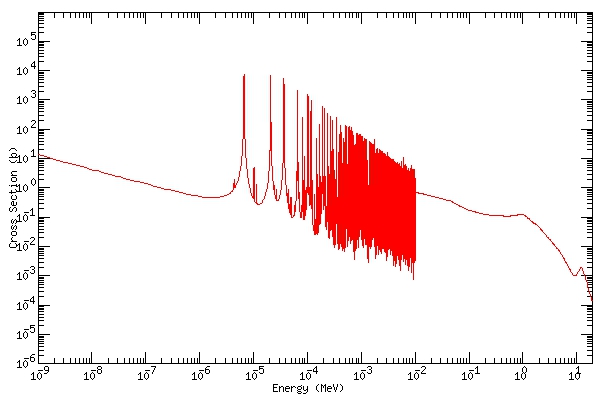
\includegraphics[width=0.75\textwidth]{ne585/fission.cross.section.jpg}
%        \caption{}
    \end{figure}
\end{frame}


\section{Fast fission factor}


\addtocounter{framenumber}{-1} 
\begin{frame}{Fast fission factor is ratio of the total number of fast and thermal neutrons produced to number produced by just thermal fission}
    \begin{enumerate}[series=outerlist,topsep=0pt,itemsep=21pt,leftmargin=*,label=(\arabic*)]
        \item[]Again, very hard to calculate
    \end{enumerate}
\end{frame}


\begin{frame}{}
    \begin{figure}
        \centering
        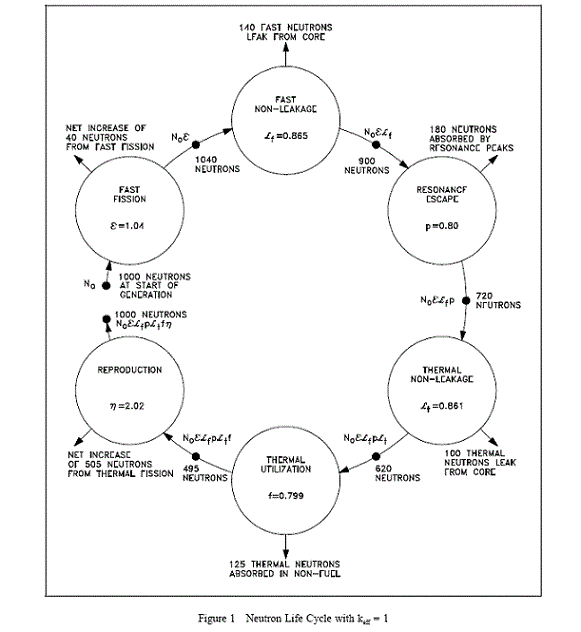
\includegraphics[width=0.55\textwidth]{ne585/neutron.generation.jpg}
%        \caption{}
    \end{figure}
\end{frame}


\section{Critical and subcritical configurations}


\addtocounter{framenumber}{-1} 
\begin{frame}{The critical mass is the minimum amount of material required to maintain $k = 1$}
    \begin{enumerate}[series=outerlist,topsep=0pt,itemsep=21pt,leftmargin=*,label=(\arabic*)]
        \item[]Critical size is determined based on material and geometry
        \item[]If the critical size of a Pu bare sphere is 10 cm, how do you make this smaller?
    \end{enumerate}

    \vspace*{\fill}

    \begin{figure}
        \centering
        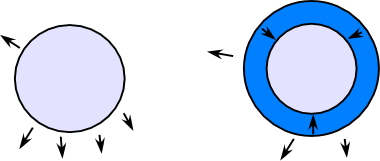
\includegraphics[width=0.55\textwidth]{ne585/reflector.jpg}
%        \caption{}
    \end{figure}
\end{frame}


\begin{frame}{$k$ is used to determine subcritical assemblies as well}
    \begin{enumerate}[series=outerlist,topsep=0pt,itemsep=21pt,leftmargin=*,label=(\arabic*)]
        \item[]Like used fuel pool storage
        \item[]Or any kind of storage
    \end{enumerate}
\end{frame}


\begin{frame}{}
    \begin{figure}
        \centering
        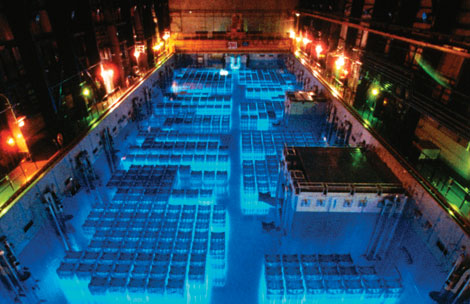
\includegraphics[width=0.75\textwidth]{ne585/used.fuel.pool.jpg}
%        \caption{}
    \end{figure}
\end{frame}


\section{Burnup}


\addtocounter{framenumber}{-1} 
\begin{frame}{Burnup is a measure of the total energy released in fission by the fuel}
    \begin{enumerate}[series=outerlist,topsep=0pt,itemsep=21pt,leftmargin=*,label=(\arabic*)]
        \item[]Typically given as GWD/MTU
        \item[]1.05 g $^{235}U$ = 1 MWD
        \item[]Also called depletion analysis
        \item[]Generation III+ designs -- 55 GWD/MTU
        \item[]Higher burnup means more fissions, more fuel consumed
        \item[]But the build up of fission product poisons means that refueling is needed
    \end{enumerate}
\end{frame}


\begin{frame}{$^{239}Pu$ is actually produced in the reactor due to $^{238}U$ neutron absorption}
    \begin{enumerate}[series=outerlist,topsep=0pt,itemsep=21pt,leftmargin=*,label=(\arabic*)]
        \item[]Quantity depends on burnup
        \item[]At the end of a fuel campaign, some Pu is fissioning as well
        \item[]This is extracted by reprocessing to make recycled \acf{mox} fuel
        \item[]Taking advantage of this, reactors can be designed to make plutonium
        \item[]Fast reactors are used
    \end{enumerate}
\end{frame}


\section{Neutron interaction rate}


\addtocounter{framenumber}{-1} 
\begin{frame}{Define energy dependent neutron interaction rate}
    \begin{equation}
        \LARGE
        F \equiv \int^\infty_0 \Sigma_T(E) \phi(E) dE
    \end{equation}

    \vspace*{\fill}

    \begin{enumerate}[series=outerlist,topsep=0pt,itemsep=21pt,leftmargin=*,label=(\arabic*)]
        \item[]Total interaction rate over all neutron energies
        \item[]Typically assume monoenergetic neutrons
        \item[]Derived in 5.1 -- whatever chapter is called `neutron diffusion'
    \end{enumerate}
\end{frame}


\section{Neutron diffusion}


\addtocounter{framenumber}{-1} 
\begin{frame}{We assume neutron diffusion follows Fick's law}
    \begin{enumerate}[series=outerlist,topsep=0pt,itemsep=21pt,leftmargin=*,label=(\arabic*)]
        \item[]Which is a good assumption because nearly everything does
        \item[]The book calls $J$ `current' 
    \end{enumerate}

    \vspace*{\fill}

    \begin{equation}
        \LARGE
        J_i \equiv -D \frac{d \phi}{di}
    \end{equation}

    \begin{equation}
        \LARGE
        D \equiv [L]
    \end{equation}

    \begin{equation}
        \LARGE
        \underline{J} \equiv \underline{\underline{D}} \nabla \phi
    \end{equation}
\end{frame}


\begin{frame}{There are conditions when Fick's law is not valid}
    \begin{enumerate}[series=outerlist,topsep=0pt,itemsep=21pt,leftmargin=*,label=(\arabic*)]
        \item[]Strongly absorbing medium
        \item[]Three mean free paths of source or medium surface
        \item[]Anisotropic scattering
    \end{enumerate}
\end{frame}


\begin{frame}{}
    \begin{figure}
        \centering
        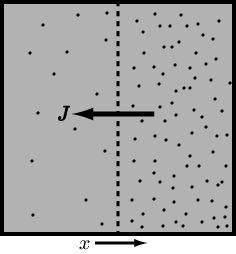
\includegraphics[width=0.35\textwidth]{ne585/current.jpg}
%        \caption{}
    \end{figure}
\end{frame}


\section{Equation of continuity}


\addtocounter{framenumber}{-1} 
\begin{frame}{Equation of continuity}
    \begin{enumerate}[series=outerlist,topsep=0pt,itemsep=21pt,leftmargin=*,label=(\arabic*)]
        \item[]Concept applied to describe many physical phenomena
        \item[]Material passing through a control volume must be accounted for
        \item[]How the control volume is defined is important
        \item[]Typically just a fixed volume
    \end{enumerate}
\end{frame}


%http://www.gammaexplorer.com/wp-content/uploads/2014/03/Introduction-to-Nuclear-Engineering-Lamarsh-3rd-Edition.pdf


\section{[rate of change of neutrons] = [production rate] - [absorption rate] - [leakage rate]}


\begin{frame}[plain]{}
    \LARGE
    \begin{equation*}
        \frac{d}{dt} \int_V n dV =
        \int_V s dV - \int_V \Sigma_A \phi dV - \int_A \underline{J} \cdot \underline{n} dA
    \end{equation*}
\end{frame}


\addtocounter{framenumber}{-2} 
\begin{frame}{\normalsize[rate of change of neutrons] = [production rate] - [absorption rate] - [leakage rate]}
    \begin{enumerate}[series=outerlist,topsep=0pt,itemsep=21pt,leftmargin=*,label=(\arabic*)]
        \item[]$\int_V n dV$ -- Total number of neutrons
        \item[]$\frac{d}{dt} \int_V n dV = \int_V \frac{\partial n}{\partial t} dV$ -- Rate of change
        \item[]$\int_V sdV$ -- Production rate
        \item[]$\int_V \Sigma_A \phi dV$ -- Absorption rate
        \item[]$\int_A \underline{J} \cdot \underline{n} dA = \int_V \nabla \underline{J} dV$ -- Leakage rate
    \end{enumerate}
\end{frame}


\begin{frame}[plain]{}
    \LARGE
    \begin{equation*}
        \int_V \frac{\partial{n}}{\partial{t}} dV = 
        \int_V s dV - \int_V \Sigma_A \phi dV - \int_V \nabla \underline{J} dV
    \end{equation*}
\end{frame}


\begin{frame}[plain]{}
    \begin{equation}
        \LARGE
        \frac{\partial{n}}{\partial{t}} = s - \Sigma_A \phi - \nabla \underline{J}
    \end{equation}
\end{frame}


\section{Diffusion equation}


\addtocounter{framenumber}{-3} 
\begin{frame}{Use the equation of continuity to obtain the diffusion equation}
    \begin{equation}
        \small
        \frac{\partial{n}}{\partial{t}} = s - \Sigma_A \phi - \nabla \underline{J}
    \end{equation}

    \begin{enumerate}[series=outerlist,topsep=0pt,itemsep=21pt,leftmargin=*,label=(\arabic*)]
        \item[]Substitute in Fick's law
    \end{enumerate}

    \vspace*{\fill}

    \begin{equation}
        \small
        D \nabla^2 \phi - \Sigma_A \phi + s = \frac{\partial{n}}{\partial{t}}
    \end{equation}

    \vspace*{\fill}

    \begin{equation}
        \small
        \phi = nv
    \end{equation}

    \begin{equation}
        \small
        D \nabla^2 \phi - \Sigma_A \phi + s = \frac{1}{v} \frac{\partial{\phi}}{\partial{t}}
    \end{equation}

    \begin{equation}
        \small
        \nabla^2 \phi - \frac{\Sigma_A}{D} \phi + \frac{s}{D} = \frac{1}{D} \frac{1}{v} \frac{\partial{\phi}}{\partial{t}}
    \end{equation}

    \begin{equation}
        \small
        \nabla^2 \phi - \frac{1}{L^2} \phi + \frac{s}{D} = \frac{1}{D} \frac{1}{v} \frac{\partial{\phi}}{\partial{t}}
    \end{equation}

    \begin{equation}
        \small
        \nabla^2 \phi - \frac{1}{L^2} \phi + \frac{s}{D} = 0
    \end{equation}
\end{frame}


\section{Diffusion length}


\addtocounter{framenumber}{-1} 
\begin{frame}{L is defined as the 'diffusion length' (5.7)}
    \begin{enumerate}[series=outerlist,topsep=0pt,itemsep=21pt,leftmargin=*,label=(\arabic*)]
        \item[]Average(ish) distance traveled by neutron before absorption
        \item[]Not quite the same as mean free path
        \item[]There are several typical solutions in 5.6 based on geometry
        \item[]$s = 0$ since the medium itself does not produce neutrons
        \item[]We are basically talking about moderator behavior
        \item[]With more math, these are valid for thermal neutrons
    \end{enumerate}
\end{frame}


\section{Group diffusion theory}


\addtocounter{framenumber}{-1} 
\begin{frame}{Neutrons have an energy distribution}
    \begin{enumerate}[series=outerlist,topsep=0pt,itemsep=17pt,leftmargin=*,label=(\arabic*)]
        \item[]Emitted in fission with continuous energy spectrum
        \item[]To get around this ranges of neutrons grouped into 'bins'
        \item[]Group diffusion theory
        \item[]Each group has averaged parameters
        \item[]Continuity equation then needs more terms
        \item[]Scatter out of the group
        \item[]Scatter into the group
        \item[]Three group diffusion, four group, five, etc.
    \end{enumerate}
\end{frame}


\begin{frame}{}
    \begin{figure}
        \centering
        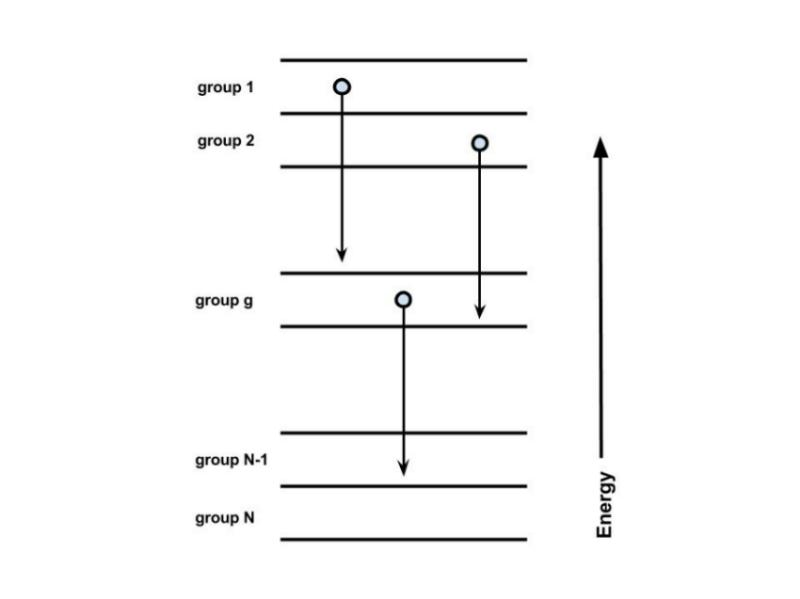
\includegraphics[width=0.75\textwidth]{ne585/groups.jpg}
%        \caption{}
    \end{figure}
\end{frame}


\begin{frame}{Group theory useful for fast neutrons and thermal neutrons}
    \begin{equation}
        \LARGE
        D_F \nabla^2 \phi_F - \Sigma_{F \rightarrow T}^S \phi_F = 0
    \end{equation}

    \begin{equation}
        \LARGE
        \nabla^2 \phi_T - \frac{1}{L^2} \phi_T + \frac{\Sigma_{F \rightarrow T}^S \phi_F}{D_T} = 0
    \end{equation}

    \vspace*{\fill}

    \begin{enumerate}[series=outerlist,topsep=0pt,itemsep=21pt,leftmargin=*,label=(\arabic*)]
        \item[]Describe in words
    \end{enumerate}
\end{frame}


\section{Nuclear reactor design}
\section{One group reactor equation}


\addtocounter{framenumber}{-2} 
\begin{frame}{Consider a bare fast reactor, homogeneous mix of fuel and coolant}
    \begin{enumerate}[series=outerlist,topsep=0pt,itemsep=21pt,leftmargin=*,label=(\arabic*)]
        \item[]Bare = no reflector
    \end{enumerate}

    \vspace*{\fill}

    \begin{equation}
        \LARGE
        D \nabla^2 \phi - \Sigma_A \phi + s = 0
    \end{equation}

    \vspace*{\fill}

    \begin{enumerate}[series=outerlist,topsep=0pt,itemsep=21pt,leftmargin=*,label=(\arabic*)]
        \item[]This time $s \neq 0$
        \item[]Cross section is for the mixture
        \item[]Source neutrons emitted due to fission not absorbed
    \end{enumerate}

    \vspace*{\fill}

    \begin{equation}
        \LARGE
        \therefore s = \eta f \Sigma_A \phi
    \end{equation}
\end{frame}


\begin{frame}{Assume an infinite reactor}
    \begin{equation}
        \LARGE
        \therefore k_\infty = \eta f
    \end{equation}

    \begin{equation}
        \LARGE
        D \nabla^2 \phi - \Sigma_A \phi + k_\infty \Sigma_A \phi = 0
    \end{equation}

    \vspace*{\fill}

    \begin{enumerate}[series=outerlist,topsep=0pt,itemsep=21pt,leftmargin=*,label=(\arabic*)]
        \item[]One group reactor equation
    \end{enumerate}

    \vspace*{\fill}

    \begin{equation}
        \LARGE
        \nabla^2 \phi + B^2 \phi = 0
    \end{equation}

    \begin{equation}
        \LARGE
        B^2 \equiv \frac{k_\infty - 1}{L^2}
    \end{equation}

    \vspace*{\fill}

    \begin{enumerate}[series=outerlist,topsep=0pt,itemsep=21pt,leftmargin=*,label=(\arabic*)]
        \item[]Someone solve for $B^2$ on the board
    \end{enumerate}
\end{frame}


\section{Buckling}


\addtocounter{framenumber}{-1} 
\begin{frame}{Solve buckling for different geometries}
    \begin{enumerate}[series=outerlist,topsep=0pt,itemsep=21pt,leftmargin=*,label=(\arabic*)]
        \item[]$B^2$ is the eigenvalue
        \item[]What does this mean?
        \item[]For a sphere -- $B^2 = (\frac{\pi}{R})^2$
        \item[]For a slab -- $B^2 = (\frac{\pi}{a})^2$
        \item[]Find the table in Lamarsh
    \end{enumerate}
\end{frame}


\begin{frame}{Buckling determines critical geometry}
    \begin{enumerate}[series=outerlist,topsep=0pt,itemsep=21pt,leftmargin=*,label=(\arabic*)]
        \item[]Solve for whatever geometry
        \item[]Integrate over the volume for power
        \item[]Use power to find the constant of integration
    \end{enumerate}

    \vspace*{\fill}

    \begin{equation}
        \LARGE
        P = E_R \Sigma_F \int \phi dV
    \end{equation}

    \begin{equation}
        \LARGE
        E_R = 3.2 \times 10^{-11} J \; per \; fission \sim 200 \; MeV
    \end{equation}
\end{frame}


\section{Leakage}


\addtocounter{framenumber}{-1} 
\begin{frame}{`Real' reactors have leakage }
    \begin{enumerate}[series=outerlist,topsep=0pt,itemsep=21pt,leftmargin=*,label=(\arabic*)]
        \item[]Neutrons either leak out or absorbed
        \item[]Even neutrons absorbed can birth the next generation
        \item[]Leaked neutrons are just gone
        \item[]$B^2 = \frac{k_\infty - 1}{L^2}$ is a necessary condition for critical reactor
        \item[]$\frac{k_\infty}{1+B^2L^2}=1$ just rearrange the equation to see the leakage term
        \item[]$k_{EFF} = k_{\infty} \cdot P_L$ is one group critical equation for a bare reactor
        \item[]With $P_L$ being a general nonleakage probability term
    \end{enumerate}
\end{frame}


\begin{frame}{But we want to account for all the neutrons that will not leak}
    \begin{enumerate}[series=outerlist,topsep=0pt,itemsep=11pt,leftmargin=*,label=(\arabic*)]
        \item[]Why
        \item[]Go back to the continuity equation
    \end{enumerate}

    \vspace*{\fill}

    \begin{equation}
        \small
        \frac{d}{dt} \int_V n dV =
        \int_V s dV - \int_V \Sigma_A \phi dV - \int_A \underline{J} \cdot \underline{n} dA
    \end{equation}

    \vspace*{\fill}

    \begin{enumerate}[series=outerlist,topsep=0pt,itemsep=11pt,leftmargin=*,label=(\arabic*)]
        \item[]Identify losses -- $\int_V \Sigma_A \phi dV$
        \item[]Identify leakage -- $- \int_V D \nabla^2 \phi dV$
        \item[]So the probability of absorption; i.e., non leakage is --
    \end{enumerate}

    \vspace*{\fill}

    \begin{equation}
        \small
        P_L \equiv \frac{\int_V \Sigma_A \phi dV}{\int_V \Sigma_A \phi dV - \int_V D \nabla^2 \phi dV}
    \end{equation}

    \begin{equation}
        \small
        \therefore P_L = \frac{\Sigma_A}{\Sigma_A + D B^2} = \frac{1}{1+B^2L^2}
    \end{equation}

    \vspace*{\fill}

    \begin{enumerate}[series=outerlist,topsep=0pt,itemsep=11pt,leftmargin=*,label=(\arabic*)]
        \item[]Because -- $- \int_V D \nabla^2 \phi dV = \int_V DB^2 \phi dV$
    \end{enumerate}
\end{frame}


\section{Criticality for thermal reactors}


\addtocounter{framenumber}{-1} 
\begin{frame}{Criticality is technically different for thermal reactors}
    \begin{equation}
       \LARGE
        \eta_T \equiv \frac{\int \eta(E) \sigma_F \phi(E) dE}{\int \eta(E) \sigma_A \phi(E) dE}
    \end{equation}

    \vspace*{\fill}

    \begin{enumerate}[series=outerlist,topsep=0pt,itemsep=11pt,leftmargin=*,label=(\arabic*)]
        \item[]Slowly varying with temperature
        \item[]Slowly varying with T
        \item[]But just look it up
        \item[]It's the same procedure = FUEL + MODERATOR
        \item[]Four factor formula is the same
        \item[]Resonance escape is an important parameter
        \item[]Why?
    \end{enumerate}
\end{frame}


\section{Two group theory}


\addtocounter{framenumber}{-1} 
\begin{frame}{Need two group theory for thermal criticality}
    \begin{enumerate}[series=outerlist,topsep=0pt,itemsep=11pt,leftmargin=*,label=(\arabic*)]
        \item[]This is like two group diffusion except the source is now nonzero
    \end{enumerate}

    \vspace*{\fill}

    \begin{equation}
        \LARGE
        D_1 \nabla^2 \phi_1 -\Sigma_1 \phi_1 + s_1=0
    \end{equation}

    \begin{equation}
        \LARGE
        D_T \nabla^2 \phi_T -\Sigma_A \phi_T + s_T=0
    \end{equation}

    \vspace*{\fill}

    \begin{enumerate}[series=outerlist,topsep=0pt,itemsep=11pt,leftmargin=*,label=(\arabic*)]
        \item[]Assume most fissions are induced by thermal neutrons
    \end{enumerate}
\end{frame}


\begin{frame}{Derive the source terms}
    \begin{enumerate}[series=outerlist,topsep=0pt,itemsep=11pt,leftmargin=*,label=(\arabic*)]
        \item[]Thermal fission neutron birth rate
    \end{enumerate}

    \vspace*{\fill}

    \begin{equation}
        \LARGE
        \eta_T f \epsilon \Sigma_A \phi_T  = \frac{k_\infty}{p} \Sigma_A \phi_T = s_1
    \end{equation}

    \vspace*{\fill}

    \begin{enumerate}[series=outerlist,topsep=0pt,itemsep=11pt,leftmargin=*,label=(\arabic*)]
        \item[]Scattered neutrons from fast group are source in thermal group
        \item[]But only those that escape resonances
    \end{enumerate}

    \vspace*{\fill}

    \begin{equation}
        \LARGE
        s_T = p \Sigma_1 \phi_1
    \end{equation}

    \vspace*{\fill}

    \begin{enumerate}[series=outerlist,topsep=0pt,itemsep=11pt,leftmargin=*,label=(\arabic*)]
        \item[]For bare thermal reactor
    \end{enumerate}
\end{frame}


\begin{frame}{}
    \begin{equation}
        \LARGE
        D_1 \nabla^2 \phi_1 - \Sigma_1 \phi_1 + \frac{k_\infty}{p} \Sigma_A \phi_T = 0
    \end{equation}

    \begin{equation}
        \LARGE
        D_T \nabla^2 \phi_T - \Sigma_A \phi_T + p \Sigma_1 \phi_1 = 0
    \end{equation}
\end{frame}


\begin{frame}{Solving it is not as hard as it might seem}
    \begin{enumerate}[series=outerlist,topsep=0pt,itemsep=11pt,leftmargin=*,label=(\arabic*)]
        \item[]Assume all group fluxes have same spatial dependence in bare reactor
    \end{enumerate}

    \vspace*{\fill}

    \begin{equation}
        \LARGE
        \phi_1 = A_1 \phi
    \end{equation}

    \begin{equation}
        \LARGE
        \phi_T = A_2 \phi
    \end{equation}

    \vspace*{\fill}

    \begin{enumerate}[series=outerlist,topsep=0pt,itemsep=11pt,leftmargin=*,label=(\arabic*)]
        \item[]Necessary condition for criticality
    \end{enumerate}

    \vspace*{\fill}

    \begin{equation}
        \LARGE
        \nabla^2 \phi + B^2 = 0
    \end{equation}
\end{frame}


\begin{frame}{Substitute these into the two group equations}
    \begin{equation}
        \LARGE
        -(D_1 B^2 + \Sigma_1) A_1 + \frac{k_\infty}{p} \Sigma_A A_2=0
    \end{equation}

    \begin{equation}
        \LARGE
        p \Sigma_1 A_1 - (D_TB^2 + \Sigma_A) A_2 = 0
    \end{equation}

    \vspace*{\fill}

    \begin{enumerate}[series=outerlist,topsep=0pt,itemsep=11pt,leftmargin=*,label=(\arabic*)]
        \item[]Apply Cramer's rule
    \end{enumerate}

    \vspace*{\fill}

    \begin{equation}
        \LARGE
        \therefore \frac{k_\infty}{(1 + B^2 L^2)(1 + B^2 \tau)} = 1
    \end{equation}

    \vspace*{\fill}

    \begin{enumerate}[series=outerlist,topsep=0pt,itemsep=11pt,leftmargin=*,label=(\arabic*)]
        \item[]Where -- $\tau \equiv \frac{D_1}{\Sigma_1}$ is the `neutron age'
    \end{enumerate}
\end{frame}


\section{Six factor formula}


\addtocounter{framenumber}{-1} 
\begin{frame}{The result is the six factor formula}
    \begin{equation}
        \LARGE
        P_F \equiv \frac{1}{1 + B^2 \tau}
    \end{equation}

    \vspace*{\fill}

    \begin{enumerate}[series=outerlist,topsep=0pt,itemsep=11pt,leftmargin=*,label=(\arabic*)]
        \item[]Probability that the fission neutron does \textit{not} escape while slowing down
    \end{enumerate}

    \vspace*{\fill}

    \begin{equation}
        \LARGE
        \therefore k = k_\infty P_L P_F
    \end{equation}

    \vspace*{\fill}

    \begin{enumerate}[series=outerlist,topsep=0pt,itemsep=11pt,leftmargin=*,label=(\arabic*)]
        \item[]Or multiply out the denominator from before
    \end{enumerate}

    \vspace*{\fill}

    \begin{equation}
        \LARGE
        \frac{k_\infty}{1 + B^2 M^2} = 1
    \end{equation}

    \vspace*{\fill}

    \begin{enumerate}[series=outerlist,topsep=0pt,itemsep=11pt,leftmargin=*,label=(\arabic*)]
        \item[]Thermal migration area
        \item[]See cases in section 6.5
    \end{enumerate}
\end{frame}


\section{Reflected reactor}


\addtocounter{framenumber}{-1} 
\begin{frame}{A reflector is added to make the core smaller}
    \begin{equation}
        \LARGE
        \nabla^2 \phi_C + B^2 \phi_C = 0 \; core
    \end{equation}

    \begin{equation}
        \LARGE
        \nabla^2 \phi_R - \frac{1}{L^2_R} \phi_C = 0 \; reflector
    \end{equation}

    \vspace*{\fill}

    \begin{enumerate}[series=outerlist,topsep=0pt,itemsep=11pt,leftmargin=*,label=(\arabic*)]
        \item[]With boundary conditions --
    \end{enumerate}

    \vspace*{\fill}

    \begin{equation}
        \LARGE
        \phi_C(R) = \phi_R(R)
    \end{equation}

    \begin{equation}
        \LARGE
        D_C \phi'_C(R) = D_R\phi'_R(R)
    \end{equation}

    \begin{equation}
        \LARGE
        \therefore BR \cdot cot(BR) - 1 = -\frac{D_R}{D_C} (\frac{R}{L_R} + 1) \; sphere
    \end{equation}
\end{frame}


\section{Reflected reactor}


\addtocounter{framenumber}{-1} 
\begin{frame}{Multigroup theory is applied in the same way (as before)}
    \begin{enumerate}[series=outerlist,topsep=0pt,itemsep=21pt,leftmargin=*,label=(\arabic*)]
        \item[]More groups gives a more accurate flux 
        \item[]Obviously gets way more complicated to solve  
        \item[]Procedure is the same
    \end{enumerate}

    \vspace*{\fill}

    \begin{enumerate}[series=outerlist,topsep=7pt,itemsep=0pt,leftmargin=*,label=(\arabic*)]
        \item[]For the two group equation --
    \end{enumerate}

    \begin{equation}
        \LARGE
        D_1 \nabla^2 \phi_1 -\Sigma_1 \phi_1 + s_1=0
    \end{equation}

    \begin{equation}
        \LARGE
        D_T \nabla^2 \phi_T -\Sigma_A \phi_T + s_T=0
    \end{equation}

    \vspace*{\fill}

    \begin{enumerate}[series=outerlist,topsep=0pt,itemsep=21pt,leftmargin=*,label=(\arabic*)]
        \item[]Now we want $N$ groups
        \item[]So we derive for an arbitrary group g which is next to a group h
    \end{enumerate}
\end{frame}


\begin{frame}{}
    \begin{figure}
        \centering
        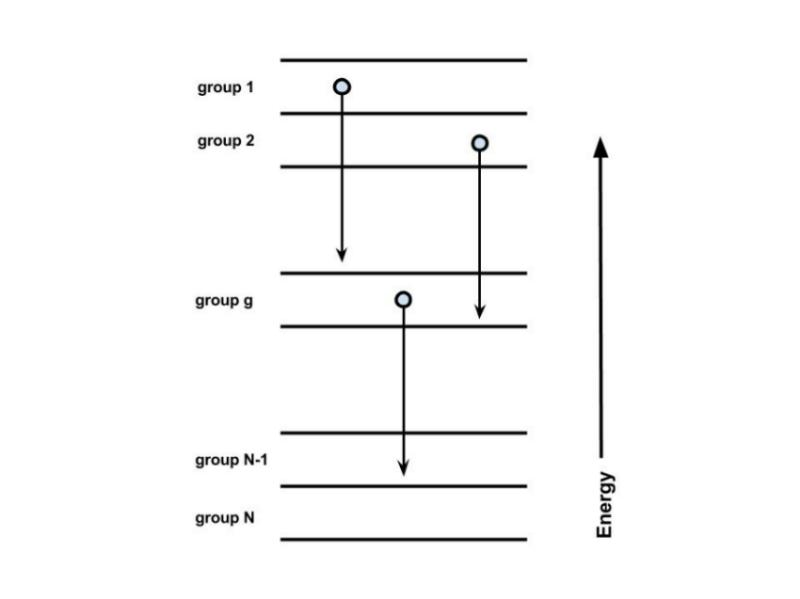
\includegraphics[width=0.75\textwidth]{ne585/groups.jpg}
%        \caption{}
    \end{figure}
\end{frame}


\begin{frame}{Multigroup theory is applied in the same way (as before)}
    \begin{enumerate}[series=outerlist,topsep=0pt,itemsep=21pt,leftmargin=*,label=(\arabic*)]
        \item[]$\Sigma_F^g$ -- group averaged fission cross section
        \item[]$\nu_g$ -- fission neutrons released per induced in the group
        \item[]$\chi_g$ -- fraction of fission neutrons emitted in the group
        \item[]$\Sigma_F^h \phi_h$ -- fission density in h group (adjacent to g)
        \item[]$\nu_h \Sigma_F^h \phi_h$ -- neutrons released from h group fissions
        \item[]$\sum \nu_h \Sigma_F^h \phi_h$ -- total neutrons emitted due to fission all groups
        \item[]$s_g = \sum_{h=1}^N \nu_h \Sigma_F^h \phi_h$ -- source
    \end{enumerate}
\end{frame}


\begin{frame}{Then put that all together}
    \begin{equation}
        \Large
        D_g \nabla^2 \phi_g - \Sigma_A^g \phi_g - \sum_{h=g + 1}^N \Sigma_{g \rightarrow h}\phi_g + \sum_{h=1}^{g-1} \Sigma_{h \rightarrow g} \phi_h + \chi_g \sum_{h=1}^N \nu_h \Sigma_F^h \phi_h = 0
    \end{equation}

    \vspace*{\fill}

    \begin{enumerate}[series=outerlist,topsep=0pt,itemsep=21pt,leftmargin=*,label=(\arabic*)]
        \item[] Can anyone do it out for 3 groups?
    \end{enumerate}
\end{frame}


\begin{frame}{}
    \begin{figure}
        \centering
        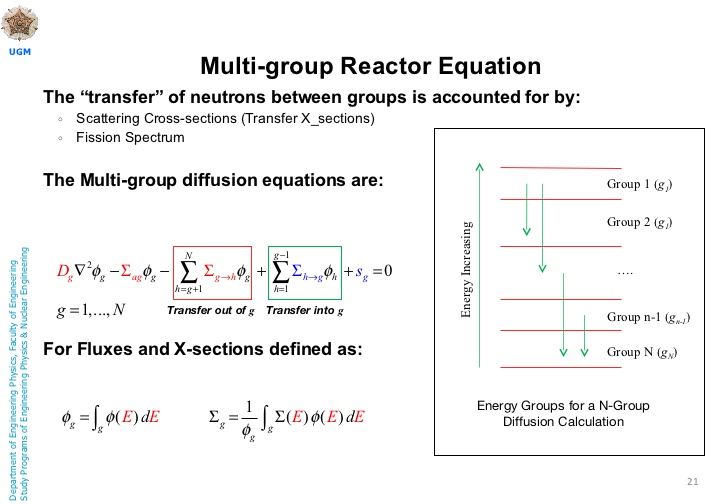
\includegraphics[width=0.75\textwidth]{ne585/group.theory.jpg}
%        \caption{}
    \end{figure}
\end{frame}


\section{Heterogeneity}


\addtocounter{framenumber}{-1} 
\begin{frame}{Unfortunately, real reactors aren't homogeneous and it makes calculating $k$ hard}
    \begin{enumerate}[series=outerlist,topsep=0pt,itemsep=21pt,leftmargin=*,label=(\arabic*)]
        \item[]Fortunately, the theory is the same
        \item[]Current \acs{lwr} fuel is enriched uranium dioxide
        \item[]And they're all thermal
    \end{enumerate}

    \vspace*{\fill}

    \begin{equation}
        \LARGE
        \eta_T = \frac{\nu^{25}\Sigma_F^{25}}{\Sigma_A^{25}+\Sigma_A^{28}}
    \end{equation}
\end{frame}


\begin{frame}{And for fuel utilization}
    \begin{enumerate}[series=outerlist,topsep=0pt,itemsep=21pt,leftmargin=*,label=(\arabic*)]
        \item[]Neutron absorption rate in fuel
    \end{enumerate}

    \vspace*{\fill}

    \begin{equation}
        \LARGE
        \int_{V_F} \Sigma_A^F \phi_T dV
    \end{equation}

    \vspace*{\fill}

    \begin{enumerate}[series=outerlist,topsep=0pt,itemsep=21pt,leftmargin=*,label=(\arabic*)]
        \item[]Neutron absorption rate in moderator
    \end{enumerate}

    \vspace*{\fill}

    \begin{equation}
        \LARGE
        \int_{V_M} \Sigma_A^M \phi_T dV
    \end{equation}
\end{frame}


\begin{frame}{And for fuel utilization}
    \begin{enumerate}[series=outerlist,topsep=0pt,itemsep=21pt,leftmargin=*,label=(\arabic*)]
        \item[]By definition --
    \end{enumerate}

    \vspace*{\fill}

    \begin{equation}
        \LARGE
        f = \frac{\Sigma_A^F \overline{\phi}_T^F V_F}{\Sigma_A^F \overline{\phi}_T^F V_F + \Sigma_A^M \overline{\phi}_T^M V_M}
    \end{equation}

    \vspace*{\fill}

    \begin{enumerate}[series=outerlist,topsep=0pt,itemsep=21pt,leftmargin=*,label=(\arabic*)]
        \item[]Hard to compute for real because of flux, so they developed approximations
    \end{enumerate}

    \vspace*{\fill}

    \begin{equation}
        \LARGE
        \frac{1}{f} = \frac{\Sigma_A^M V_M}{\Sigma_A^F V_F} \cdot F + E
    \end{equation}

    \vspace*{\fill}

    \begin{enumerate}[series=outerlist,topsep=0pt,itemsep=21pt,leftmargin=*,label=(\arabic*)]
        \item[]Of course they had to use F to confuse everyone
        \item[]Lattice constants, Bessel functions p264 for F,E
        \item[]p265 for lattice and unit cell
    \end{enumerate}
\end{frame}


\begin{frame}{Wigner-Seitz equivalent cylindrical cell}
    \begin{figure}
        \centering
        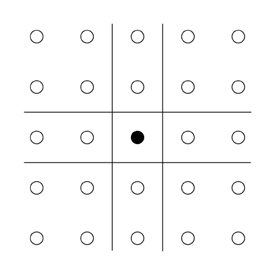
\includegraphics[width=0.45\textwidth]{ne585/lattice.unit.cell.jpg}
%        \caption{}
    \end{figure}
\end{frame}


\begin{frame}{Then for resonance escape}
    \begin{equation}
        \LARGE
        p = e^{-\frac{N_F V_F I}{\xi_M \Sigma_S^M V_M}}
    \end{equation}

    \vspace*{\fill}

    \begin{enumerate}[series=outerlist,topsep=0pt,itemsep=21pt,leftmargin=*,label=(\arabic*)]
        \item[]$N_F$ is the fuel atom density
        \item[]$\xi_M$ is the average increase in lethargy in the moderator
        \item[]$I = A + \frac{C}{\sqrt{a\rho}}$ is the resonance integral
        \item[]$A,C$ are constants, $a$ is fuel rod radius, $\rho$ is fuel density -- p266
        \item[]So basically there are a bunch of semi empirical expressions needed
        \item[]Very typical in engineering
    \end{enumerate}
\end{frame}


\section{Reactor kinetics}


\addtocounter{framenumber}{-1} 
\begin{frame}{Reactor kinetics is about what happens when the reactor shuts down or starts up}
    \begin{equation}
        \LARGE
        \therefore \frac{\partial{n}}{\partial{t}} \neq 0
    \end{equation}

    \vspace*{\fill}

    \begin{enumerate}[series=outerlist,topsep=0pt,itemsep=21pt,leftmargin=*,label=(\arabic*)]
        \item[]Changes in temperature affect changes in neutron multiplication
        \item[]Reactor is initially loaded with more than the minimum critical mass due to burnup
        \item[]Criticality affected by fission products
        \item[]Many are gaseous and have to be trapped
    \end{enumerate}
\end{frame}


\section{Prompt neutrons}


\addtocounter{framenumber}{-1} 
\begin{frame}{There are different kinds of neutrons to account for}
    \begin{enumerate}[series=outerlist,topsep=0pt,itemsep=21pt,leftmargin=*,label=(\arabic*)]
        \item[]Prompt neutrons are emitted at the instant of fission
        \item[]Delayed neutrons emitted after the fission event
        \item[]These control reactor kinetics
    \end{enumerate}
\end{frame}


\begin{frame}{Prompt neutron lifetime is the average time between emission and absorption}
    \begin{enumerate}[series=outerlist,topsep=0pt,itemsep=21pt,leftmargin=*,label=(\arabic*)]
        \item[]Time for neutron to slow to thermal is small compared to time as thermal
        \item[]Prompt neutron lifetime $l_P$ = mean diffusion time $t_D$ in the infinite thermal reactor
    \end{enumerate}
\end{frame}


\begin{frame}{Reason out the reactor physics to derive $t_D$}
    \begin{enumerate}[series=outerlist,topsep=0pt,itemsep=21pt,leftmargin=*,label=(\arabic*)]
        \item[]Neutron travels an absorption mean free path before actually being absorbed
        \item[]Energy dependent to start
    \end{enumerate}

    \vspace*{\fill}

    \begin{equation}
        \LARGE
        t(E) = \frac{\lambda_A(E)}{v(E)}
    \end{equation}

    \begin{equation}
        \LARGE
        t(E) = \frac{1}{\Sigma_A(E)v(E)}
    \end{equation}

    \begin{equation}
        \LARGE
        t_D \equiv \overline{t(E)}
    \end{equation}

    \vspace*{\fill}

    \begin{enumerate}[series=outerlist,topsep=0pt,itemsep=21pt,leftmargin=*,label=(\arabic*)]
        \item[]Assuming Maxwell in the thermal region -- $\frac{1}{v}$
        \item[]$t(E)$ isn't energy dependent anymore because $E_0 = 0.0253 eV$ and $v_0 = 2200 m/s$
    \end{enumerate}
\end{frame}


\begin{frame}{Reason out the reactor physics to derive $t_D$}
    \begin{equation}
        \LARGE
        \therefore t_D = \frac{\sqrt{\pi}}{2} \cdot \frac{1}{\Sigma_A v_T}
    \end{equation}

    \vspace*{\fill}

    \begin{enumerate}[series=outerlist,topsep=0pt,itemsep=21pt,leftmargin=*,label=(\arabic*)]
        \item[]For fuel and moderator --
    \end{enumerate}

    \vspace*{\fill}

    \begin{equation}
        \LARGE
        t_D = \frac{\sqrt{\pi}}{2 v_T} \cdot \frac{1}{\Sigma_A^F + \Sigma_A^M}
    \end{equation}

    \vspace*{\fill}

    \begin{enumerate}[series=outerlist,topsep=0pt,itemsep=21pt,leftmargin=*,label=(\arabic*)]
        \item[]Or --
    \end{enumerate}

    \begin{equation}
        \LARGE
        t_D = \frac{\sqrt{\pi}}{2 v_T} \cdot \frac{\Sigma_A^M}{\Sigma_A^M} \cdot \frac{1}{\Sigma_A^F + \Sigma_A^M}
    \end{equation}
\end{frame}


\begin{frame}{Reason out the reactor physics to derive $t_D$}
    \begin{equation}
        \LARGE
        t_D = \frac{\sqrt{\pi}}{2 v_T \Sigma_A^M} \cdot \frac{\Sigma_A^M}{\Sigma_A^F + \Sigma_A^M}
    \end{equation}

    \begin{equation}
        \LARGE
        \therefore t_D = \frac{\sqrt{\pi}}{2 v_T \Sigma_A^M}(1 - f)
    \end{equation}

    \vspace*{\fill}

    \begin{enumerate}[series=outerlist,topsep=0pt,itemsep=21pt,leftmargin=*,label=(\arabic*)]
        \item[]$\sim 10^4 \; s$ for water
        \item[]Prompt neutron lifetime is much shorter in fast reactors than thermal $\sim 10^{-7} \; s$
    \end{enumerate}
\end{frame}


\begin{frame}{What role do neutrons play in reactor kinetics?}
    \begin{enumerate}[series=outerlist,topsep=0pt,itemsep=21pt,leftmargin=*,label=(\arabic*)]
        \item[]Consider an infinite thermal reactor with only prompt neutrons
        \item[]Prompt neutron lifetime $l_P$ then is time between successive neutron generations
        \item[]Absorption of a neutron at $t=t_0$ means absorption of $k_\infty$ neutrons at $t=t_0+l_P$
    \end{enumerate}
\end{frame}


\begin{frame}{How to we derive a measure of this time?}
    \begin{equation}
        \LARGE
        N_F(t + l_P) = k_\infty N_F(t)
    \end{equation}

    \vspace*{\fill}

    \begin{enumerate}[series=outerlist,topsep=0pt,itemsep=21pt,leftmargin=*,label=(\arabic*)]
        \item[]Take a Taylor expansion of the left side
    \end{enumerate}

    \vspace*{\fill}

    \begin{equation}
        \LARGE
        N_F(t + l_P) \approx N_F(t) + l_P\frac{dN_F(t)}{dt}
    \end{equation}

    \vspace*{\fill}

    \begin{enumerate}[series=outerlist,topsep=0pt,itemsep=21pt,leftmargin=*,label=(\arabic*)]
        \item[]Substitute back in
    \end{enumerate}

    \vspace*{\fill}

    \begin{equation}
        \LARGE
        \frac{dN_F(t)}{dt} = \frac{k_\infty - 1}{l_P}N_F(t)
    \end{equation}
\end{frame}


\section{Reactor period -- Prompt}


\addtocounter{framenumber}{-1} 
\begin{frame}{How to we derive a measure of this time?}
    \begin{equation}
        \LARGE
        N_F(t)=N_F(0)e^{\frac{t}{T}}
    \end{equation}

    \begin{equation}
        \LARGE
        T = \frac{l_P}{k_\infty - 1}
    \end{equation}

    \vspace*{\fill}

    \begin{enumerate}[series=outerlist,topsep=0pt,itemsep=21pt,leftmargin=*,label=(\arabic*)]
        \item[]$T$ is called the reactor period (in the absence of delayed neutrons)
        \item[]What is this telling us?
        \item[]What is the period physically describing?
    \end{enumerate}
\end{frame}


\section{Picture break}


\addtocounter{framenumber}{-1} 
\begin{frame}{}
    \begin{figure}
        \centering
        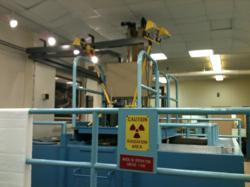
\includegraphics[width=0.45\textwidth]{ne585/wpi.bridge.jpg}
%        \caption{}
    \end{figure}
\end{frame}


\begin{frame}{}
    \begin{figure}
        \centering
        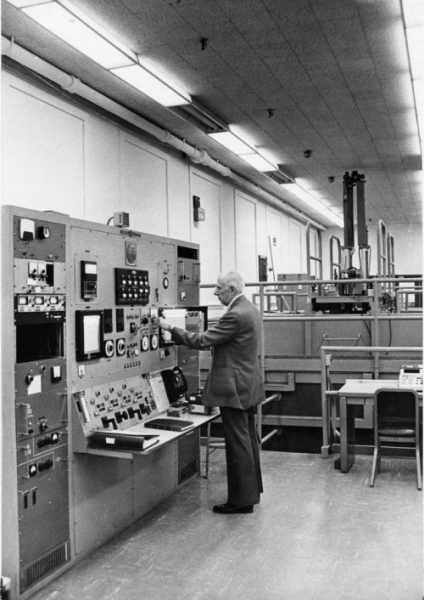
\includegraphics[width=0.35\textwidth]{ne585/wpi.control.panel.jpg}
%        \caption{}
    \end{figure}
\end{frame}


\section{Delayed neutrons}


\addtocounter{framenumber}{-1} 
\begin{frame}{\href{https://www.nrc.gov/docs/ML1214/ML12142A098.pdf}{Delayed neutrons control reactor operation}}
    \begin{enumerate}[series=outerlist,topsep=0pt,itemsep=21pt,leftmargin=*,label=(\arabic*)]
        \item[]Six groups of delayed neutron precursors with characteristic half life
        \item[]Fission products that produce neutrons as part of decay process
        \item[]For infinite homogeneous thermal reactor (not necessarily critical) one group of delayed neutrons
        \item[]The diffusion equation for thermal neutrons is (5.21)
    \end{enumerate}

    \vspace*{\fill}

    \begin{equation}
        \LARGE
        \frac{dn}{dt} = s_T - \Sigma_A \phi_T
    \end{equation}

    \vspace*{\fill}

    \begin{enumerate}[series=outerlist,topsep=0pt,itemsep=21pt,leftmargin=*,label=(\arabic*)]
        \item[]Assume thermal flux is independent of position
    \end{enumerate}
\end{frame}


\section{Point kinetics equations}


\addtocounter{framenumber}{-1} 
\begin{frame}{Deriving rate of change for delayed neutrons}
    \begin{enumerate}[series=outerlist,topsep=0pt,itemsep=21pt,leftmargin=*,label=(\arabic*)]
        \item[]From 5.9 based on Maxwellian distribution
    \end{enumerate}

    \vspace*{\fill}

    \begin{equation}
        \LARGE
        \phi_T = \frac{2}{\sqrt{\pi}} nv_T
    \end{equation}

    \begin{equation}
        \LARGE
        l_P \approx t_D = \frac{\sqrt{\pi}}{2} \cdot \frac{1}{\Sigma_A v_T}
    \end{equation}

    \begin{equation}
        \LARGE
        \frac{dn}{dt} = s_T - \Sigma_A \phi_T
    \end{equation}

    \vspace*{\fill}

    \begin{enumerate}[series=outerlist,topsep=0pt,itemsep=21pt,leftmargin=*,label=(\arabic*)]
        \item[]Substitute back in
    \end{enumerate}

    \vspace*{\fill}

    \begin{equation}
        \LARGE
        l_P\frac{d\phi_T}{dt}=\frac{s_T}{\Sigma_A}-\phi_T
    \end{equation}
\end{frame}


\begin{frame}{Now derive $s_T$}
    \begin{enumerate}[series=outerlist,topsep=0pt,itemsep=21pt,leftmargin=*,label=(\arabic*)]
        \item[]The source has two contributions -- Prompt and delayed
        \item[]If $\beta \equiv$ fraction of fission neutrons that are delayed, then the prompt contribution --
    \end{enumerate}

    \vspace*{\fill}

    \begin{equation}
        \LARGE
        s_T^P = (1 - \beta) k_\infty \Sigma_A \phi_T
    \end{equation}
\end{frame}


\begin{frame}{Delayed neutrons slow down quick after emission}
    \begin{equation}
        \LARGE
        s_T^D=p\lambda C
    \end{equation}

    \vspace*{\fill}

    \begin{enumerate}[series=outerlist,topsep=0pt,itemsep=21pt,leftmargin=*,label=(\arabic*)]
        \item[]$p \equiv$ resonance escape and $\lambda C$ is decay of precursor (like Bateman)
        \item[]This means the source is based on the production from the precursor and the probability it escaped through the resonance region
    \end{enumerate}
\end{frame}


\begin{frame}{Combining everything}
    \begin{equation}
        \LARGE
        l_P \frac{d\phi_T}{dt} = (1-\beta) k_\infty \Sigma_A \phi_T + \frac{p}{\Sigma_A} \lambda C - \phi_T
    \end{equation}

    \vspace*{\fill}

    \begin{enumerate}[series=outerlist,topsep=0pt,itemsep=21pt,leftmargin=*,label=(\arabic*)]
        \item[]Rate of change of thermal flux based on one group of delayed neutrons
        \item[]$C$ is the precursor concentration
        \item[]We need another equation
    \end{enumerate}
\end{frame}


\begin{frame}{Derive the precursor equation}
    \begin{enumerate}[series=outerlist,topsep=0pt,itemsep=21pt,leftmargin=*,label=(\arabic*)]
        \item[]Fission neutron production rate --
    \end{enumerate}

    \vspace*{\fill}

    \begin{equation}
        \LARGE
        \eta_T \epsilon f \Sigma_A \phi_T = \frac{1}{p} k_\infty \Sigma_A \phi_T
    \end{equation}

    \vspace*{\fill}

    \begin{enumerate}[series=outerlist,topsep=0pt,itemsep=21pt,leftmargin=*,label=(\arabic*)]
        \item[]Delayed neutron production rate is then --
    \end{enumerate}

    \vspace*{\fill}

    \begin{equation}
        \LARGE
        \beta \cdot \frac{1}{p} k_\infty \Sigma_A \phi_T
    \end{equation}

    \begin{equation}
        \LARGE
        \therefore \frac{dC}{dt} = \beta \cdot \frac{1}{p} k_\infty \Sigma_A \phi_T - \lambda C
    \end{equation}
\end{frame}


\begin{frame}{Point kinetics describes reactor transient behavior}
    \begin{equation}
        \LARGE
        l_P \frac{d\phi_T}{dt} = (1-\beta) k_\infty \Sigma_A \phi_T + \frac{p}{\Sigma_A} \lambda - \phi_T
    \end{equation}

    \begin{equation}
        \LARGE
        \frac{dC}{dt} = \beta \cdot \frac{1}{p} k_\infty \Sigma_A \phi_T -\lambda C
    \end{equation}

    \vspace*{\fill}

    \begin{enumerate}[series=outerlist,topsep=0pt,itemsep=21pt,leftmargin=*,label=(\arabic*)]
        \item[]Leo M. Bobek, R. A. Borrelli, PLC-based reactivity measurements using inverse point kinetics, Transactions of the American Nuclear Society, 74, Annual meeting of the American Nuclear Society, 16-20 June, 1996, Reno, Nevada.
    \end{enumerate}
\end{frame}


\section{How is a solution obtained?}


\addtocounter{framenumber}{-1} 
\begin{frame}{Solve the system simultaneously}
    \begin{enumerate}[series=outerlist,topsep=0pt,itemsep=21pt,leftmargin=*,label=(\arabic*)]
        \item[]Assume $k_\infty = 1$ at $t = 0$
        \item[]Step change then made to change $k_\infty$
        \item[]Assume --
    \end{enumerate}

    \vspace*{\fill}

    \begin{equation}
        \LARGE
        \phi = A e^{\omega t} \rightarrow \frac{d\phi}{dt} = \omega A e^{\omega t}
    \end{equation}

    \begin{equation}
        \LARGE
        C = C_0 e^{\omega t} \rightarrow \frac{dC}{dt} = \omega C_0 e^{\omega t}
    \end{equation}

    \vspace*{\fill}

    \begin{enumerate}[series=outerlist,topsep=0pt,itemsep=21pt,leftmargin=*,label=(\arabic*)]
        \item[]Substitute --
    \end{enumerate}

    \vspace*{\fill}

    \begin{equation}
        \LARGE
        \omega C_0 e^{\omega t}=(\beta \frac{1}{p} k_\infty \Sigma_A)(A e^{\omega t})-\lambda (C_0 e^{\omega t})
    \end{equation}
\end{frame}


\begin{frame}{\href{https://uidaho.pressbooks.pub/nuclearengineering/chapter/math-skills/}{Solve the system simultaneously}}
    \begin{enumerate}[series=outerlist,topsep=0pt,itemsep=21pt,leftmargin=*,label=(\arabic*)]
        \item[]Continuing gives us reactivity equation for one group of delayed neutrons
    \end{enumerate}

    \vspace*{\fill}

    \begin{equation}
        \LARGE
        \rho = \frac{\omega l_P}{1+\omega l_P} + \frac{\omega}{1+\omega l_p} \frac{\beta}{\omega+\lambda}
    \end{equation}

    \begin{equation}
        \LARGE
        \rho \equiv \frac{k-1}{k}
    \end{equation}

    \vspace*{\fill}

    \begin{enumerate}[series=outerlist,topsep=0pt,itemsep=21pt,leftmargin=*,label=(\arabic*)]
        \item[]What is the range of $\rho$?
    \end{enumerate}

    \vspace*{\fill}

    \begin{equation}
        \LARGE
        \rho = \frac{\omega l_P}{1 + \omega l_P} + \frac{\omega}{1 + \omega l_p} \sum_{i=1}^6 {\frac{\beta_i}{\omega + \lambda_i}}
    \end{equation}
\end{frame}


\section{Reactor period -- Delayed}


\addtocounter{framenumber}{-1} 
\begin{frame}{We still need to figure out $\omega$}
    \begin{enumerate}[series=outerlist,topsep=0pt,itemsep=21pt,leftmargin=*,label=(\arabic*)]
        \item[]Figure 7.1
    \end{enumerate}

    \vspace*{\fill}

    \begin{equation}
        \LARGE
        \phi_T = A_1 e^{\omega_1 t} + A_2 e^{\omega_2 t}
    \end{equation}

    \vspace*{\fill}

    \begin{enumerate}[series=outerlist,topsep=0pt,itemsep=21pt,leftmargin=*,label=(\arabic*)]
        \item[]For either $\rho < 1$ or $\rho > 1$ the second term dies out
    \end{enumerate}

    \vspace*{\fill}

    \begin{equation}
        \LARGE
        \phi_T \rightarrow e^{\omega_1 t}
    \end{equation}

    \vspace*{\fill}

    \begin{enumerate}[series=outerlist,topsep=0pt,itemsep=21pt,leftmargin=*,label=(\arabic*)]
        \item[]This gives reactor period as --
    \end{enumerate}

    \vspace*{\fill}

    \begin{equation}
        \LARGE
        T = \frac{1}{\omega_1}
    \end{equation}
\end{frame}


\section{Prompt critical}


\addtocounter{framenumber}{-1} 
\begin{frame}{Let's look at the prompt critical reactor state}
    \begin{enumerate}[series=outerlist,topsep=0pt,itemsep=21pt,leftmargin=*,label=(\arabic*)]
        \item[]If the reactor would be critical only on prompt neutrons --
    \end{enumerate}

    \vspace*{\fill}

    \begin{equation}
        \LARGE
        (1-\beta) k = 1
    \end{equation}

    \vspace*{\fill}

    \begin{enumerate}[series=outerlist,topsep=0pt,itemsep=21pt,leftmargin=*,label=(\arabic*)]
        \item[]The period is very short and you can't control the reactor
        \item[]The reactivity corresponding to prompt critical is just --
    \end{enumerate}

    \vspace*{\fill}

    \begin{equation}
        \LARGE
        \rho = \beta
    \end{equation}

    \vspace*{\fill}

    \begin{enumerate}[series=outerlist,topsep=0pt,itemsep=21pt,leftmargin=*,label=(\arabic*)]
        \item[]What is $k$ for this condition for $^{235}U$?
        \item[]See table 7.2
        \item[]Although, can you really go prompt critical?
    \end{enumerate}
\end{frame}


\begin{frame}{We need the reactivity insertion to actually control the reactor}
    \begin{enumerate}[series=outerlist,topsep=0pt,itemsep=21pt,leftmargin=*,label=(\arabic*)]
        \item[]If there isn't much to `give', there isn't proper reactor kinetic control
        \item[]Units of dollars are used (because of course they are) to normalize reactivity per prompt critical
        \item[]\href{https://www.osti.gov/servlets/purl/1374731}{South Korean research reactor experiment at \acs{atr}}
    \end{enumerate}
\end{frame}


\begin{frame}{Insertion of reactivity gives a sudden rise in the flux and vice versa}
    \begin{equation}
        \LARGE
        \phi_T = A_1 e^{\omega_1 t} + A_2 e^{\omega_2 t}
    \end{equation}

    \vspace*{\fill}

    \begin{enumerate}[series=outerlist,topsep=0pt,itemsep=21pt,leftmargin=*,label=(\arabic*)]
        \item[]With 7 exponentials if all groups are concerned 
        \item[]Those terms die away liked we talked about before
        \item[]Then stable period is achieved
        \item[]We want to know what that rise/drop is (prompt jump approximation)
        \item[]The rapid die-away gives sudden rise/drop to the flux before stability
    \end{enumerate}
\end{frame}


\begin{frame}{Assume precursor concentrations do not change over the rise/drop}
    \begin{equation}
        \LARGE
        \therefore \frac{dC}{dt} = 0
    \end{equation}

    \begin{equation}
        \LARGE
        C = \beta \frac{1}{p} \frac{1}{\lambda} \Sigma_A \phi_T^0
    \end{equation}

    \vspace*{\fill}

    \begin{enumerate}[series=outerlist,topsep=0pt,itemsep=21pt,leftmargin=*,label=(\arabic*)]
        \item[]Substitute --
    \end{enumerate}

    \vspace*{\fill}

    \begin{equation}
        \LARGE
        l_P \frac{d\phi_T}{dt} = (1-\beta) k_\infty \Sigma_A \phi_T + \frac{p}{\Sigma_A} \lambda C - \phi_T
    \end{equation}
\end{frame}


\begin{frame}{Solve for flux}
    \begin{equation}
        \LARGE
        l_P \frac{d\phi_T}{dt} =(1-\beta) k_\infty \Sigma_A \phi_T + \frac{p}{\Sigma_A} \lambda C - \phi_T
    \end{equation}

    \begin{equation}
        \LARGE
        l_P \frac{d\phi_T}{dt} = [(1-\beta)k_\infty-1] \phi_T + \beta \phi_T^0
    \end{equation}

    \begin{equation}
        \LARGE
        \phi_T = \phi_T^0 e^{\frac{(1-\beta) k_\infty-1} {l_P}t} + \frac{\beta \phi_T^0}{1 - (1-\beta) k_\infty}[1 - e^{\frac{(1-\beta) k_\infty - 1} {l_P}t}]
    \end{equation}
\end{frame}


\begin{frame}{For reactivity less than prompt critical the exponentials die out}
    \begin{equation}
        \LARGE
        \phi_T = \frac{\beta}{1 - (1-\beta) k_\infty} \phi_T^0
    \end{equation}

    \vspace*{\fill}

    \begin{enumerate}[series=outerlist,topsep=0pt,itemsep=21pt,leftmargin=*,label=(\arabic*)]
        \item[]Then --
    \end{enumerate}

    \vspace*{\fill}

    \begin{equation}
        \LARGE
        \phi_T = \frac{\beta (1 - \rho)}{\beta - \rho} \cdot \phi_T^0
    \end{equation}
\end{frame}


\begin{frame}{Figure 7.3 p287}
    \begin{figure}
        \centering
        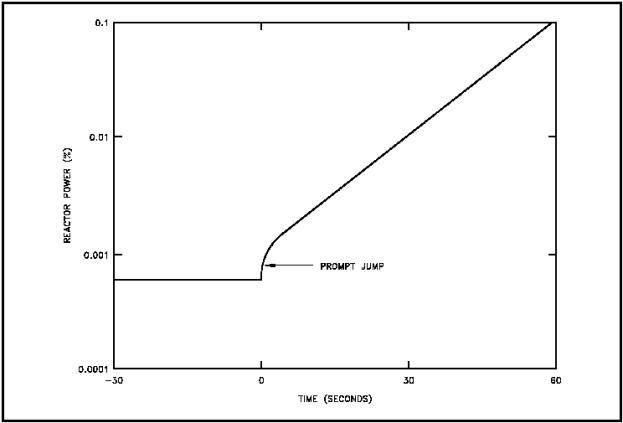
\includegraphics[width=0.75\textwidth]{ne585/prompt.jump.jpg}
%        \caption{}
    \end{figure}
\end{frame}


\section{What does this mean?}


\addtocounter{framenumber}{-1} 
\begin{frame}{What does this mean?}
    \begin{enumerate}[series=outerlist,topsep=0pt,itemsep=21pt,leftmargin=*,label=(\arabic*)]
        \item[]What happens when there is positive reactivity insertion?
        \item[]What happens with a negative reactivity insertion?
    \end{enumerate}
\end{frame}


\section{Control rod worth}


\addtocounter{framenumber}{-1} 
\begin{frame}{What does this mean?}
    \begin{enumerate}[series=outerlist,topsep=0pt,itemsep=18pt,leftmargin=*,label=(\arabic*)]
        \item[]Addition of a control rod to a finite geometry reactor requires solving the reactor equation twice (coupled) because buckling is different given the insertion of a rod(s)
        \item[]Usual diffusion theory doesn't work
        \item[]Solving this analytically can be overly much
        \item[]From a design standpoint, the arrangement of rods needs to let the neutron flux be as uniform as possible over the core
        \item[]Boric acid is often introduced into the coolant to affect criticality
        \item[]Changes thermal utilization ($f$)
        \item[]Figure 7.10 experiment -- Rod worth curve
    \end{enumerate}
\end{frame}


\section{Picture break}


\addtocounter{framenumber}{-1} 
\begin{frame}{}
    \begin{figure}
        \centering
        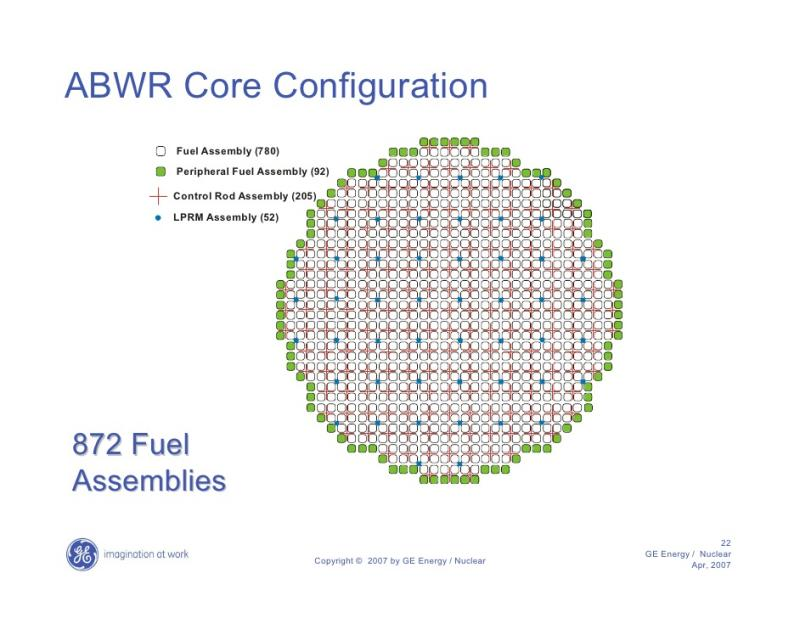
\includegraphics[width=0.75\textwidth]{ne585/abwr.jpg}
%        \caption{}
    \end{figure}
\end{frame}


\begin{frame}{}
    \begin{figure}
        \centering
        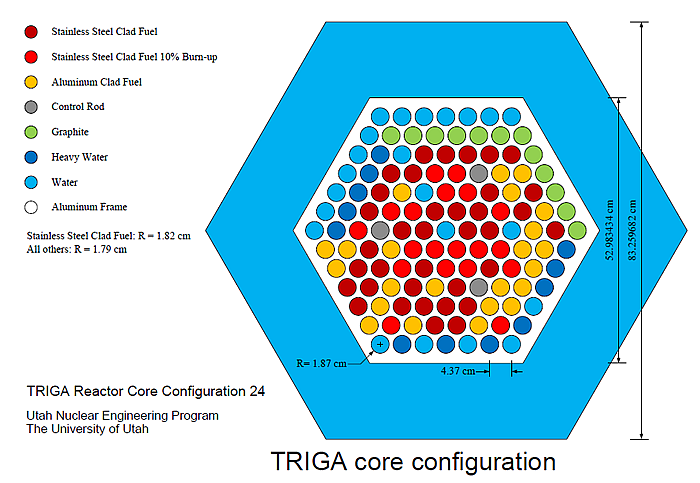
\includegraphics[width=0.75\textwidth]{ne585/triga.jpg}
%        \caption{}
    \end{figure}
\end{frame}


\section{Temperature coefficient}


\addtocounter{framenumber}{-1} 
\begin{frame}{Many parameters that contribute to neutron multiplication are temperature dependent which changes reactivity in the system}
    \begin{equation}
        \LARGE
        \alpha \equiv \frac{d\rho}{dT} \approx \frac{1}{k} \frac{dk}{dT}
    \end{equation}

    \vspace*{\fill}

    \begin{enumerate}[series=outerlist,topsep=0pt,itemsep=21pt,leftmargin=*,label=(\arabic*)]
        \item[]With a positive coefficient, and increase in temperature leads to meltdown, because of uncontrollable feedback loop
        \item[]Increase in $T$ = increase in $k$ and vice versa for positive coefficient
        \item[]With negative coefficient the feedback returns the reactor to its original state
        \item[]Increase in $T$ = decrease in $k$
        \item[]Cannot obtain a license otherwise
    \end{enumerate}
\end{frame}


\section{Doppler broadening}


\addtocounter{framenumber}{-1} 
\begin{frame}{Doppler broadening is the change in resonance with temperature}
    \begin{enumerate}[series=outerlist,topsep=0pt,itemsep=21pt,leftmargin=*,label=(\arabic*)]
        \item[]Basically about trying to describe changes due to thermal motion of atoms with temperature
        \item[]Changes the resonance region and affects cross sections (absorption)
        \item[]Resonance peaks broaden due to vibration of nuclei
        \item[]$^{238}U$ absorbs more neutrons without causing fission as reactor temperature increases
        \item[]Increase in reactor temperature leads to a fall in reactivity
        \item[]Increase in reactor temperature increases resonance absorption, decreases $k$
    \end{enumerate}
\end{frame}


\begin{frame}{So, the point is to apply the \href{https://uidaho.pressbooks.pub/nuclearengineering/chapter/nuclear-reactor-kinetics-2/}{Doppler effect} to assure a negative coefficient}
    \begin{enumerate}[series=outerlist,topsep=0pt,itemsep=21pt,leftmargin=*,label=(\arabic*)]
        \item[]Affects real time control of the reactor
        \item[]Figure 7.12 on p309
        \item[]Inverse relationship with flux
    \end{enumerate}
\end{frame}


\begin{frame}{}
    \begin{figure}
        \centering
        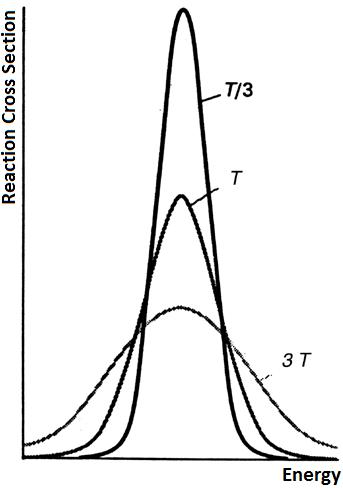
\includegraphics[width=0.40\textwidth]{ne585/resonance.jpg}
%        \caption{}
    \end{figure}
\end{frame}


\section{Void coefficient}


\addtocounter{framenumber}{-1} 
\begin{frame}{The void coefficient describes change in reactivity to void fraction}
    \begin{equation}
        \LARGE
        \alpha \equiv \frac{d\rho}{dx}
    \end{equation}

    \vspace*{\fill}

    \begin{enumerate}[series=outerlist,topsep=0pt,itemsep=15pt,leftmargin=*,label=(\arabic*)]
        \item[]Void basically means the volume occupied by vapor in the coolant upon boiling
        \item[]Void fraction increases reactivity, power, boiling, uncontrolled feedback loop
        \item[]So, void coefficient needs to be negative (why?)
        \item[]Voids affect moderator/coolant density
        \item[]More voids decrease density
        \item[]Important for BWR control
        \item[]Increases leakage
    \end{enumerate}
\end{frame}


\section{Fission product poisons}


\addtocounter{framenumber}{-1} 
\begin{frame}{Fission product poisons accumulate with burnup}
    \begin{figure}
        \centering
        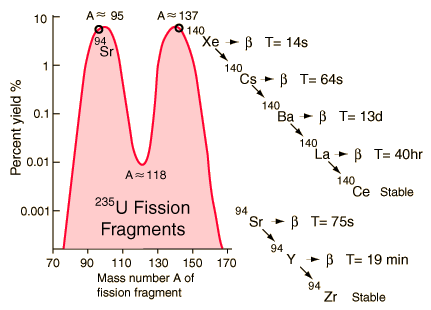
\includegraphics[width=0.65\textwidth]{ne585/fission.product.yield.jpg}
%        \caption{}
    \end{figure}
\end{frame}


\begin{frame}{Fission products absorb neutrons}
    \begin{enumerate}[series=outerlist,topsep=0pt,itemsep=21pt,leftmargin=*,label=(\arabic*)]
        \item[]What does this do to the multiplication factor? 
    \end{enumerate}

    \vspace*{\fill}

    \begin{equation}
        \LARGE
        f = \frac{\Sigma_A^F}{\Sigma_A^F+\Sigma_A^M+\Sigma_A^P}
    \end{equation}

    \vspace*{\fill}

    \begin{enumerate}[series=outerlist,topsep=0pt,itemsep=21pt,leftmargin=*,label=(\arabic*)]
        \item[]Using the definition of neutron multiplication
    \end{enumerate}

    \vspace*{\fill}

    \begin{equation}
        \LARGE
        \rho = -\frac{\Sigma_A^P}{\Sigma_F} \cdot \frac{1}{\nu p \epsilon}
    \end{equation}

    \vspace*{\fill}

    \begin{enumerate}[series=outerlist,topsep=0pt,itemsep=21pt,leftmargin=*,label=(\arabic*)]
        \item[]What does this mean for reactor operation?
    \end{enumerate}
\end{frame}


\begin{frame}{$^{135}Xe$ is a huge poison because $\Sigma_A \approx 2 \times 10^6 \; b$}
    \begin{enumerate}[series=outerlist,topsep=0pt,itemsep=21pt,leftmargin=*,label=(\arabic*)]
        \item[]That's a lot of cows
        \item[]Xenon is produced by $^{135}I$ decay but also a fission product
    \end{enumerate}

    \vspace*{\fill}

    \begin{equation}
        \LARGE
        \frac{dI}{dt} = \gamma_I\Sigma_F\phi_T - \lambda_I I
    \end{equation}

    \begin{equation}
        \LARGE
        \frac{dX}{dt} = \lambda_I I + \lambda_X\Sigma_F\phi_T - \sigma_A\phi_T X - \lambda_X X
    \end{equation}

    \vspace*{\fill}

    \begin{enumerate}[series=outerlist,topsep=0pt,itemsep=21pt,leftmargin=*,label=(\arabic*)]
        \item[]On shutdown, flux is zero and production of Xe is only due to $I$ decay
        \item[]Reactor cannot be restarted (unless you fool it with a cold start) until all the $Xe$ decays
        \item[]Due to the high negative reactivity
    \end{enumerate}
\end{frame}


\begin{frame}{}
    \begin{figure}
        \centering
        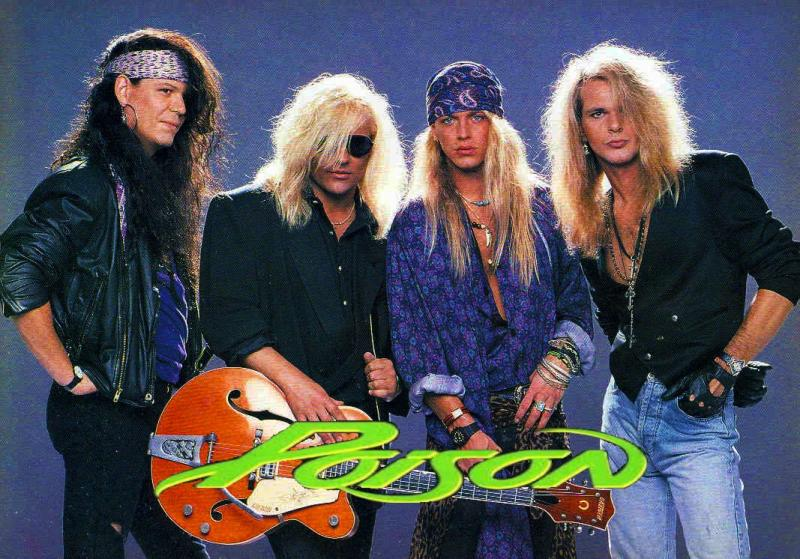
\includegraphics[width=0.75\textwidth]{ne585/poison.jpg}
%        \caption{}
    \end{figure}
\end{frame}


\begin{frame}{This is basically what goes into making a power reactor}
    \begin{enumerate}[series=outerlist,topsep=0pt,itemsep=21pt,leftmargin=*,label=(\arabic*)]
        \item[]Fortunately, we have codes to do this for us
        \item[]But understanding what is going on and being able to explain it is critical (*rimshot*) to being a nuclear engineer even if it's not your primary field
    \end{enumerate}
\end{frame}


%\begin{frame}[plain]{}
%    \centering\LARGE\textbf{Heat removal}\\
%    \centering\LARGE\textbf{Chapter 8}
%\end{frame}


%\addtocounter{framenumber}{-1} 
%\begin{frame}{Amount of heat produced be the amount of heat transferred out of core in unit time}
%    \begin{enumerate}[series=outerlist,topsep=0pt,itemsep=21pt,leftmargin=*,label=(\arabic*)]
%        \item[]Power deposited to fuel must equal the power transferred from the fuel rod to the coolant
%        \item[]Power transferred from fuel rods to the coolant (plus the power deposited directly to the coolant) must equal the power transferred by coolant out of the core
%        \item[]Cannot have fuel temperature increase without taking heat away because it will melt
%    \end{enumerate}
%\end{frame}


%\begin{frame}[plain]{}
%    \centering\LARGE\textbf{Heat removal rate}
%\end{frame}


%\addtocounter{framenumber}{-1} 
%\begin{frame}{The coolant takes away all the heat from the reactor to make electricity}
%    \begin{enumerate}[series=outerlist,topsep=0pt,itemsep=21pt,leftmargin=*,label=(\arabic*)]
%        \item[]There are limits on bulk temperature though because the fuel would melt
%    \end{enumerate}
%
%    \vspace*{\fill}
%
%    \begin{equation}
%        \LARGE
%        q = \omega \int_{T_I}^{T_O} c_P(T) dT
%    \end{equation}
%
%    \vspace*{\fill}
%
%    \begin{enumerate}[series=outerlist,topsep=0pt,itemsep=21pt,leftmargin=*,label=(\arabic*)]
%        \item[]For constant pressure and $\omega$ is coolant flow rate
%    \end{enumerate}
%\end{frame}


%\begin{frame}[plain]{}
%    \centering\LARGE\textbf{Heat production rate}
%\end{frame}


%\addtocounter{framenumber}{-1} 
%\begin{frame}{Spatial distribution of fission energy depends on reactor structure}
%    \begin{enumerate}[series=outerlist,topsep=0pt,itemsep=21pt,leftmargin=*,label=(\arabic*)]
%        \item[]Most of recoverable fission energy is deposited in the fuel
%        \item[]The rest in the coolant/moderator (20 MeV)
%    \end{enumerate}
%
%    \vspace*{\fill}
%
%    \begin{equation}
%        \LARGE
%        q^{'''}(\underline{r}) = E_D \int_0^{\infty} \Sigma_F(E) \phi(\underline{r},E) dE
%    \end{equation}
%
%    \vspace*{\fill}
%
%    \begin{enumerate}[series=outerlist,topsep=0pt,itemsep=21pt,leftmargin=*,label=(\arabic*)]
%        \item[]Power density in fuel
%        \item[]$E_D$ = energy deposited locally in the fuel per fission
%    \end{enumerate}
%\end{frame}


%\begin{frame}{Spatial distribution of fission energy depends on reactor structure}
%    \begin{equation}
%        \LARGE
%        q^{'''}(\underline{r}) = E_D \int_0^{\infty} \Sigma_F(E) \phi(\underline{r},E) dE
%    \end{equation}
%
%    \vspace*{\fill}
%
%    \begin{enumerate}[series=outerlist,topsep=0pt,itemsep=21pt,leftmargin=*,label=(\arabic*)]
%        \item[]Then look up the flux based on geometry
%        \item[]A single fuel rod would just be a finite cylinder
%        \item[]Similar model for gamma ray heat
%        \item[]Cooling after shutdown is important due to fission product heat
%    \end{enumerate}
%\end{frame}


%\begin{frame}[plain]{}
%    \centering\LARGE\textbf{Conduction and convection}
%\end{frame}


%\addtocounter{framenumber}{-1} 
%\begin{frame}{Heat is removed from the reactor by conduction and convection}
%    \begin{enumerate}[series=outerlist,topsep=0pt,itemsep=21pt,leftmargin=*,label=(\arabic*)]
%        \item[]Heat transfer from fuel rod to rod surface by conduction
%        \item[]Heat at rod surface transferred into the coolant and moved out of system by convection
%    \end{enumerate}
%\end{frame}


%\begin{frame}[plain]{}
%    \centering\LARGE\textbf{Conduction}
%\end{frame}


%\addtocounter{framenumber}{-1} 
%\begin{frame}{We use Fourier's law for conduction}
%    \begin{equation}
%        \LARGE
%        \underline{q}^{''} = -k\nabla T
%    \end{equation}
%
%    \vspace*{\fill}
%
%    \begin{enumerate}[series=outerlist,topsep=0pt,itemsep=21pt,leftmargin=*,label=(\arabic*)]
%        \item[]Based on heat conservation through a control volume
%        \item[]Heat flow out of the surface --
%    \end{enumerate}
%
%    \vspace*{\fill}
%
%    \begin{equation}
%        \LARGE
%        \int_A \underline{q}^{''} \cdot \underline{n}dA = \int_V \nabla \underline{q}^{''} dV
%    \end{equation}
%
%    \vspace*{\fill}
%
%    \begin{enumerate}[series=outerlist,topsep=0pt,itemsep=21pt,leftmargin=*,label=(\arabic*)]
%        \item[]Heat production --
%    \end{enumerate}
%
%    \vspace*{\fill}
%
%    \begin{equation}
%        \LARGE
%        \int_V \underline{q}^{'''} dV
%    \end{equation}
%\end{frame}


%\begin{frame}{Then we get the steady state heat equation}
%    \begin{equation}
%        \LARGE
%        k \nabla^2 T \underline{q}^{'''} = 0
%    \end{equation}
%
%    \vspace*{\fill}
%
%    \begin{enumerate}[series=outerlist,topsep=0pt,itemsep=21pt,leftmargin=*,label=(\arabic*)]
%        \item[]And then solve for different geometries and sources
%        \item[]With no heat sources --
%    \end{enumerate}
%
%    \vspace*{\fill}
%
%    \begin{equation}
%        \LARGE
%        \nabla^2 T = 0
%    \end{equation}
%
%    \vspace*{\fill}
%
%    \begin{enumerate}[series=outerlist,topsep=0pt,itemsep=21pt,leftmargin=*,label=(\arabic*)]
%        \item[]This is Laplace's equation used for all sorts of modeling
%    \end{enumerate}
%\end{frame}
%
%
%\begin{frame}[plain]{}
%    \centering\LARGE\textbf{Convection}
%\end{frame}
%
%
%\addtocounter{framenumber}{-1} 
%\begin{frame}{Newton's law describes heat transfer from a solid to a moving fluid}
%    \begin{equation}
%        \LARGE
%        q^{''} = h(T_C-T_B)
%    \end{equation}
%
%    \begin{equation}
%        \LARGE
%        q = hA(T_C-T_B)
%    \end{equation}
%
%    \vspace*{\fill}
%
%    \begin{enumerate}[series=outerlist,topsep=0pt,itemsep=21pt,leftmargin=*,label=(\arabic*)]
%        \item[]Similar to Ohm's law where hA = `thermal resistance'
%        \item[]Can have spatial dependence $T(z)$ for a rod
%        \item[]Heat flow into a coolant channel can be derived based on this
%    \end{enumerate}
%\end{frame}


%\begin{frame}[plain]{}
%    \centering\LARGE\textbf{Dimensionless heat transfer numbers}
%\end{frame}


%\addtocounter{framenumber}{-1} 
%\begin{frame}{Coolant flows under turbulent conditions to maximize heat transfer}
%    \begin{equation}
%        \LARGE
%        Re \equiv \frac{D_E v \rho}{\mu} \; Re > 10^4
%    \end{equation}
%
%    \begin{equation}
%        \LARGE
%        Nu \equiv \frac{hD_E}{k} \; convective:conductive
%    \end{equation}
%
%    \begin{equation}
%        \LARGE
%        Pr \equiv \frac{c_p\mu}{k} \; viscous; diff:thermal\; diff
%    \end{equation}
%
%    \begin{equation}
%        \LARGE
%        Nu = CRe^mPr^n
%    \end{equation}
%
%    \vspace*{\fill}
%
%    \begin{enumerate}[series=outerlist,topsep=0pt,itemsep=21pt,leftmargin=*,label=(\arabic*)]
%        \item[]Design relationship for convective heat transfer
%        \item[]Heat transfer for liquid metals is mostly by conduction
%    \end{enumerate}
%\end{frame}


%\begin{frame}[plain]{}
%    \centering\LARGE\textbf{Boiling}
%\end{frame}


%\addtocounter{framenumber}{-1} 
%\begin{frame}{For boiling coolant, different story}
%    \begin{enumerate}[series=outerlist,topsep=0pt,itemsep=15pt,leftmargin=*,label=(\arabic*)]
%        \item[]Bubbles of vapor form on the fuel rods (nucleate boiling)
%        \item[]Process continues to bulk boiling where steam is produced
%        \item[]Heat transfer is more efficient but void fraction increases
%        \item[]Different boiling regimes affect reactor operation
%        \item[]If film channels form on the rods, heat transfer decreases
%        \item[]Heat is confined within the rods
%        \item[]Positive feedback leads to partial meltdown
%        \item[]Need to stay in the nucleate regime  
%        \item[]Empirical, thermodynamic correlations have been developed
%    \end{enumerate}
%\end{frame}


%\begin{frame}[plain]{}
%    \centering\LARGE\textbf{Meltdown}
%\end{frame}


%\addtocounter{framenumber}{-1} 
%\begin{frame}{Integrity of the cladding contains the fission products}
%    \begin{enumerate}[series=outerlist,topsep=0pt,itemsep=21pt,leftmargin=*,label=(\arabic*)]
%        \item[]Melting fuel would expand and crack the cladding
%        \item[]Fission products (gas) would be released; e.g., Fukushima
%        \item[]Melting point depends on burnup 
%        \item[]Generation IV fuel has higher melting points than Generation II/III/III+
%        \item[]Have to be concerned about solid phase change of uranium (crystal structure)
%        \item[]Leads to fuel expansion
%    \end{enumerate}
%\end{frame}


\begin{frame}[plain]{}
    \begin{figure}
        \centering
        \includegraphics[width=0.75\textwidth]{ne585/4-final.jpg}
%        \caption{}
    \end{figure}
\end{frame}


%%%%%%%
%\begin{frame}{}
%    \begin{columns}
%
%        \begin{column}{0.50\textwidth}
%            \begin{enumerate}[series=outerlist,topsep=0pt,itemsep=21pt,leftmargin=*,label=(\arabic*)]
%                \item[]
%                \item[]
%            \end{enumerate}
%        \end{column}
%
%        \begin{column}{0.50\textwidth}
%            \begin{enumerate}[series=outerlist,topsep=0pt,itemsep=21pt,leftmargin=*,label=(\arabic*)]
%                \item[]
%                \item[]
%            \end{enumerate}
%        \end{column}
%
%    \end{columns}
%\end{frame}

%    \begin{figure}
%        \centering
%        \includegraphics[width=0.75\textwidth]{wsc.png}
%        \caption{\acs{wsc}}
%    \end{figure}


%\begin{frame}{References}
%    \bibliographystyle{nsf}
%    \footnotesize
%    \bibliography{references}
%\end{frame}
%%%%%%%


\end{document}
